\chapter{多体微扰理论}

\section{Reyleigh-\sch 微扰理论}
\label{sec6.1}
本节推导标准的Reyleigh-\sch 微扰论的表达式. 这些式子都是一般性的,既能用于单粒子系统也能用于N-粒子系统. 现设想要求解如下本征值问题:
\begin{align}
\label{6.1}
\hs \ket{\Phi_i}=(\hs_0+\vs)\ket{\Phi_i}=\mathscr{E}_i\ket{\Phi_i}
\end{align}
而且已经知道$\hs_0$的本征函数和本征值:
\begin{align}
\hs_0\ket{\Psi_i^{(0)}}=E_i^{(0)}\ket{\Psi_i^{(0)}}\qquad\text{或}\qquad \hs_0\ket{i}=E_i^{(0)}\ket{i}
\end{align}
其中为简洁用$\ket{i}$代表$\ket{\Psi_i}$. 若微扰$\vs$在某种程度上很小,那么可以期望的是,$\ket{\Phi_i},\mathscr{E}$会很接近$\ket{i},E_i^{(0)}$. 现在想找出一种方法,能使$\hs_0$的本征函数和本征值系统地逼近总哈密顿量$\hs$的本征函数和本征值。为此,我们引入一个阶参数,之后再令其等于1,有:
\begin{align}
\hs=\hs_0+\lambda\vs
\end{align}
现将精确的本证函数与本征值展开成$\lambda$的Taylor级数,
\begin{subequations}
	\begin{align}
	\es &= E_i^{(0)} + \lambda E_i^{(1)} + \lambda^2 E_i^{(2)} + \cdots\\
	\ket{\Phi_i} &= \ket{i} + \lambda \ket{\Psi_i^{(1)}} + \lambda^2 \ket{\Psi_i^{(2)}} + \cdots
	\end{align}
\end{subequations}
称$E_i^{(n)}$为$n$阶能量.现在的问题是如何将精确量用零阶能量以及微扰算符$\vs$在未微扰波函数间的矩阵元$\braket{i|\vs|j}$表达出来.

现在设$\hs$的波函数已归一化:$\braket{i|i}=1$, 且在$\ket{\Phi_i}$上乘上一个因子以使其满足等式$\braket{i|\Phi_i}=1$. 这种处理叫作"中间归一化", 并且, 除非$\ket{i}$与$\ket{\Phi_i}$正交, 否则总可以进行中间归一化. 将(6.4b)左乘$\bra{i}$, 得到
\begin{align}
\braket{i|\Phi_i}=\braket{i|i}+\lambda\braket{i|\Phi_i^{(1)}}+\lambda^2\braket{i|\Phi_i^{(2)}} + \cdots = 1
\end{align}
上面的方程对于所有的$\lambda$都成立($\lambda$不等于1时也成立), 那么就有
\begin{align}
\braket{i|\Psi_i^{(n)}} = 0\, n=1,2,3,\cdots
\end{align}
将(6.4a,6.4b)带入\ref{6.1}, 得到:
\begin{align*}
(\hs_0&+\lambda\vs)(\ket{i}+\lambda\ket{\Psi_i^{(1)}} + \lambda^2 \ket{\Psi_i^{(2)}} +\cdots )\\
&=(E_i^{(0)} + \lambda E_i^{(1)} + \lambda^2 E_i^{(2)} + \lambda^2 E_i^{(2)} + \cdots )
\end{align*}
因为$\lambda^n$的系数对应相等,我们有
\begin{subequations}
	\begin{align}
\hs_0\ket{i}&=E_i^{(0)}\ket{i}\, n=0\\
\hs_0\ket{\Psi_i^{(1)}} + \vs\ket{i}& = E_i^{0}\ket{\Psi_i^{(1)}} + E_i^{(1)}\ket{i}\, n=1 \\
\hs_0\ket{\Psi_i^{(2)}}+\vs\ket{\Psi_i^{(1)}} & = E_i^{(0)}\ket{\Psi_i^{(2)}} + E_i^{(1)}\ket{\Psi_i^{(1)}} + E_i^{(2)}\ket{i} \, n=2 \\
\hs_0\ket{\Psi_i^{(3)}}+\vs\ket{\Psi_i^{(2)}} & = E_i^{(0)}\ket{\Psi_i^{(3)}} + E_i^{(1)}\ket{\Psi_i^{(2)}} + E_I^{(2)}\ket{\Psi_i^{(2)}} +E_i^{(3)}\ket{i}\, n=1
	\end{align}
\end{subequations}
等等. 每个式子左乘$\ket{i}$, 由正交关系\ref{6.6}可得如下各阶能量:
\begin{subequations}
\begin{align}
E_I^{(0)} &= \braket{i|\hs|i} \\
E_I^{(1)} &= \braket{i|\vs|i} \\
E_I^{(2)} &= \braket{i|\hs|\Psi_i^{(1)}} \\
E_I^{(3)} &= \braket{i|\hs|\Psi_i^{(2)}}
\end{align}
\end{subequations}
剩下的事情就是从(6.7)解出$\ket{\Psi_i^{(n)}}$, 然后用(6.8)确定$n$阶能量.

先来看(6.7b), 由它来解出一阶波函数$\ket{\Psi_i^{(1)}}$. 此式可重写为
\begin{align}
(E_i^{(0)} - \hs_0 )\ket{\Psi_i^{(1)}} = (\vs - \braket{i|\vs|i})\ket{i}
\end{align}
上式不再是一个本征方程, 而成为了一个非齐次微分方程(更广义地, 成为了积分微分方程). 解该方程的一种办法是将$\ket{\Psi_i^{(1)}}$用$\hs$的本征函数展开(因为$\hs_0$的本征函数是完备的):
\begin{align*}
\ket{\Psi_i^{(1)}} = \sum_n c_n^{(1)}\ket{n}
\end{align*}
又因$\hs_0$的本征函数是正交的, 将上式左乘$\bra{n}$ 得到
\begin{align*}
\bra{n|\Psi_i^{(1)}} = c_n^{(1)}
\end{align*}
由(6.6)可知, $c_i^{(1)}=0$, 所以有
\begin{align}
\ket{\Psi_i^{1}} = \sideset{}{'}\sum_n\ket{n}\bra{n}\ket{\Psi_i^{(1)}}
\end{align}
求和号上的一撇代表不包括$n=i$的项. (6.9)左乘$\bra{n}$, 并注意到零阶波函数的正交性, 就可以得到:
\begin{align}
(E_i^{(0)} - E_n^{0} )\braket{n|\Psi_i^{(1)}} = \braket{n|\vs|i}
\end{align}
为得到二阶能量, 将(6.10)带入(6.8c)可以得到:
\begin{align*}
E_i^{(2)} = \braket{i|\vs|\Psi_i^{(1)}} = \sideset{}{'}\sum_n\braket{i|\vs|n}\braket{n|\Psi_i^{(1)}}
\end{align*}
使用(6.11)可以求出$\braket{n|\Psi_i^{(1)}}$, 所以最终有
\begin{align}
E_i^{(2)} = \sideset{}{'}\sum_n\frac{\braket{i|\vs|n}\braket{n|\vs|i}}{E_i^{(0)} - E_n^{(0)}}
\end{align}
这就是二阶能量的表达式.

若想到三阶能量$E_i^{(3)}$, 可以使用相同的手续. 首先将二阶波函数展开为
\begin{align}
\ket{\Psi_i^{(2)}} = \sideset{}{'}{\sum_n}\ket{n}\braket{n|\Psi_i^{(2)}}
\end{align}
然后荣$\bra{n}$去乘(6.7c), 得到
\begin{align}
(E_i^{(0)} -E_n^{(0)} )\braket{n|\Psi_i^{(2)}} = \braket{n|\vs|\Psi_i^{(1)}} - E_i^{(1)}\braket{n|\Psi_i^{(1)}}
\end{align}
将(6.8d)(6.13)(6.14)组合可得
\begin{align*}
E_i^{(3)} & = \braket{i|\vs|\Psi_i^{(2)}}\\
		  & = \sideset{}{'}{\sum_n}\braket{i|\vs|n}\braket{n|\Psi_i^{(2)}}\\
		  & =\sideset{}{'}{\sum_n}\frac{\braket{i|\vs|n}\braket{n|\vs|\Psi_I^{(1)}}}{E_i^{(0)} - E_N^{(0)}} - E_i^{(1)} \sideset{}{'}{\sum_n}\frac{\braket{i|\vs|n}\braket{n|\Psi_i^{(1)}}}{E_i^{(0)} - E_n^{(0)} }
\end{align*}
最后再将(6.10)(6.11)插入, 就得到
\begin{align}
E_I^{(3)} & =\sideset{}{'}{\sum_{mn}}\frac{\braket{i|\vs|n}\braket{n|\vs|m}\braket{m|\vs|i} }{(E_i^{(0)} -E_n^{(0)})(E_i^{(0)} - E_m^{(0)} )  } - E_i^{(1)} \sideset{}{'}{\sum_n} \frac{\left| \braket{i|\vs|n} \right|^2}{(E_i^{(0)} -E_n^{(0)} )^2}\notag\\
& = A_i^{(3)} + B_i^{(3)}
\label{6.15}
\end{align}
这就是三阶能量.

此处给出这种办法的一个应用. 考虑一个体系, 该体系仅右边两个状态$\ket{I},\ket{II}$, 都是哈密顿量$\hs$的本征函数:
\begin{align*}
\hs\ket{I} = \es_1\ket{I} \qquad \hs\ket{II} = \es_2\ket{II}
\end{align*}
假设
\begin{align*}
\hs=\hs_0+\vs
\end{align*}
而且知道$\hs_0$的本征函数:
\begin{align*}
\hs_0\ket{1} = E_1^{(0)}\ket{1}\qquad \hs_0\ket{2} = E_2^{(0)}\ket{2}
\end{align*}
现在想得到精确的基态能量$\es_1$. 假设零阶态非简并, 而且$E_1^{(0)}$是较低的能量(即$E_1^{(0)} < E_2^{(0)}$). 我们先用精确的办法得出解, 然后再用微扰理论求解, 最后比较这两个结果. 为求解方程
\begin{align}
\hs\ket{\Phi}=\es\ket{\Phi}
\end{align}
写出如下展开
\begin{align}
\ket{\Phi} = c_1\ket{1} + c_2\ket{2}
\end{align}
由此得到
\begin{align}
\begin{bmatrix}
E_1^{(0)} + \braket{1|\vs|1} & \braket{1|\vs|2}\\
\braket{2|\vs|1}			& E_2^{0} + \braket{2|\vs|2}
\end{bmatrix}
\begin{bmatrix}
c_1\\c_2
\end{bmatrix}
=
\es\begin{bmatrix}
c_1\\c_2
\end{bmatrix}
\end{align}
为简化记号, 令$\braket{1|\vs|1}=V_{11},\braket{1|\vs|2}=V_{12},\braket{2|\vs|1}=V_{21},\braket{2|\vs|2}=V_{22}$. 此矩阵较小的那个本征值为:
\begin{align}
\es_1 = \frac{1}{2} \left\{  E_1^{(0)} + V_{11} + E_2^{(0)} + V_{22} - \left[ (E_1^{(0)} -E_{2}^{(0)} + V_{11} - V_{22})^2 +4V_{12}V_{21} \right]^{1/2}      \right\}\tag{6.19a}
\addtocounter{equation}{1}
\end{align}

现将$\es_1$按微扰矩阵元展成Taylor级数.  为此, 将每个微扰矩阵元都乘以系数$\lambda$:
\begin{align}
\es_1 = \frac{1}{2} \left\{  E_1^{(0)} + \lambda V_{11} + E_2^{(0)} + \lambda V_{22} - \left[ (E_1^{(0)} -E_{2}^{(0)} + \lambda(V_{11} - V_{22}))^2 +4\lambda^2 V_{12}V_{21} \right]^{1/2}      \right\}\tag{6.19b}
\end{align}
然后将$\es_1$展成$\lambda$的Taylor级数.

此处需要两个等式:
\begin{align}
	(1+x)^{1/2} =& 1 + \frac{1}{2} x - \frac{1}{8} x^2 + \cdots\\
	(1-x)^{-1}  =& 1 +x +x^2 +x^3+\cdots
\end{align}
先来将$\es_1$写成:
\begin{align*}
\es_1 = & \frac{1}{2} \Bigg\{ E_1^{(0)} + \lambda V_{11} + E_2^{(0)} + \lambda V_{22} + (E_1^{(0)} -E_2^{(0)} +\lambda(V_{11} - V_{22}) ) \\
\times & \left[1 + \frac{4\lambda^2V_{11}V_{22}}{(E_1^{(0)}  - E_2^{(0)} + \lambda(V_{11}-V_{22}) )^2} \right]^{1/2}
     \Bigg\}
\end{align*}
请注意, 我们从平方根中提出了因子$(E_1^{(0)}) - E_2^{(2)} +\lambda(V_{11}-V_{22}) $, 此处假设它是负的, 因为$E_1^{(0)}<E_2^{(0)}$, 而且扰动(即$\vs$)是小的.

首先展开平方根(略), 然后展开$(E_1^{(0)}-E_2^{(0)} + \lambda(V_{11}-V_{22}))^{-1}$如下:
\begin{align*}
	\frac{1}{(E_1^{(0)}-E_2^{(0)} + \lambda(V_{11}-V_{22})} & =\frac{1}{E_1^{(0)} - E_2^{(0) }}\cdot \frac{1}{1+\frac{\lambda(V_{11}-V_{22}) }{E_1^{0} -E_2^{(0)} }}\\
		& = \frac{1}{E_1^{(0)} - E_2^{(0)}} - \frac{\lambda(V_{11}-V_{22}) }{E_1^{0} -E_2^{(0)} }+\cdots
\end{align*}
可以证明
\begin{align}
\es_1 = E_1^{(1)} + \lambda E_1^{(1)} + \lambda^2 E_1^{(2)} + \lambda^3 E_1^{(3)} + E\lambda^4 E_1^{(4)} + \cdots
\end{align}
其中
\begin{subequations}
	\begin{align}
	E_1^{(1)} &= V_{11} \\
	E_1^{(2)} &= \frac{V_{12}V_{21}}{E_1^{0} - E_2^{(0)}} \\
	E_1^{(3)} &= \frac{V_{12} V_{22} V_{21} }{(E_1^{(0)} - E_2^{(0)})^2} - \frac{V_{12} V_{21} V_{11} }{ (E_1^{(0)} - E_2^{(0)})^2 }\\
	E_1^{(4)} &= \frac{V_{12} V_{21} V_{11}^2 }{(E_1^{(0)} - E_2^{(0)})^3} - \frac{2 V_{12} V_{22} V_{21} V_{11} }{(E_1^{(0)} - E_2^{(0)})^3} + \frac{V_{12} V_{22}^2 V_{21} }{(E_1^{(0)} - E_2^{(0)})^3} + \frac{ (V_{12} V_{21})^2 }{(E_1^{(0)} - E_2^{(0)})^3}
	\end{align}
\end{subequations}

最终我们能看到,由RS微扰理论出发所得的一、二、三阶能量的公式[(6.8b)(6.12)(6.15)]与以上式中的$E_1^{(n)}\,(n=1,2,3)$相等. 为理解这一点,只需注意到两态问题中中仅有一个中间态$\ket{n} = \ket{2}$. 由于微扰理论的公式是由Taylor展开所得,出现这样的对应也是可期的。

\section{RS微扰论的图表示}
\label{sec6.2}
上节末尾我们已经看到, 即使是最简单的两态问题,其高阶能量公式也相当复杂。本章的主要目标就是将Hartree-Fock基态作为零阶态来得到相关能的微扰展开公式. 在这种情况下, 高阶能量的表达式愈将复杂. 因此若能找到某种相对简单的方法, 将高阶展开中的各项归类并表示出来, 那将再好不过. 本节来介绍一种图形化方法, 用图形表示微扰展开. 我们并不会严格地推导图形微扰论, 而是从一个简单的例子开始, 推测出微扰展开和一组含义明确的图形之间的对应关系. 然后我们再``猜出"将图形转化为数学式子的规则, 并展示其正确性.接下来会推广之前的图形及规则, 并在每一步都检查有图形所得的式子和直接推导所得式子之间的一致性. 用这种办法是望读者能习惯并认可这些图形.

微扰展开的图形表示首先出现在量子电动力学中. Feynman首创了这种办法, 并在他的Nobel讲座上介绍了其想法的演变发展. 此处引用他的几句话``我其余的工作就是发展了计算技巧, 用图形来帮助人们更快地分析微扰论. 这个工具最初基本上是猜出来的.."``即使是从物理学家的层面来讲, 我也并未证明这些规则和方程可以通过传统的电动力学得到, 但是从平时的``胡搞"中我已经知道, 所有这些东西和传统的电动力学毫无二致."

\subsection{两态系统的图微扰论}
上节考察了两态问题, 并得到了基态本征值表达式, 此处介绍该表达式中各项所对应的图形表示. 首先, 用一个点来表示微扰$\vs$ :
\[\begin{tikzpicture}
\draw (0,0)[<->] node[left]{$\vs$} -- (1,0)node[right]{$\bullet$};
\end{tikzpicture}
\]
两个零阶态$\ket{1}$, $\ket{2}$由向上和向下的箭头表示:
\begin{align*}
\ket{1}\longleftrightarrow\quad \begin{tikzpicture}[scale=.5,baseline=(current bounding box.center)]
\path[draw=blue,postaction={on each segment={mid arrow}}] (0,0)--(0,-1);
\end{tikzpicture}
\\
\ket{2}\longleftrightarrow\quad \begin{tikzpicture}[draw=blue,scale=.5,baseline=(current bounding box.center)]
	\path[draw=blue,postaction={on each segment={mid arrow}}] (0,-1)--(0,0);
	\end{tikzpicture}
\end{align*}
箭头向下的线叫作``空穴"线, 箭头向上的线叫粒子线. 这些术语暂时不重要, 此处只是提早介绍一下. 由这些定义, 可以画出一些简单的图形来代表$\vs$的矩阵元:


\[
\begin{array}{ccc}
\braket{1|\vs|1}&=V_{11}\longleftrightarrow &\tikz[baseline=(current bounding box.center)]{\path[draw=blue,postaction={on each segment={mid arrow}}] (0,0.33)--node[right]{1}(0,0)--node[right]{1}(0,-.33);}
\\[5mm]
\braket{1|\vs|2}&=V_{12}\longleftrightarrow &\tikz[scale=.5,baseline=(current bounding box.center)]{\path[draw=blue,postaction={on each segment={mid arrow}}] (-0.77,0.77)--(0,0)--(.77,.77);}
\\[5mm]
\braket{1|\vs|2}&=V_{12}\longleftrightarrow &
\\[5mm]
\braket{1|\vs|1}&=V_{11}\longleftrightarrow &
\end{array}
\]
总之, 每个点上都有一线段进入, 有一线段穿出. 对应的矩阵元就是$\braket{\text{穿入线的标签}| \vs |\text{穿出线的标签} }$.

回忆$n$阶能量表达式中的各项: $n=1,2,3,4$分子都是$n$个$\vs$矩阵元的乘积. 每个矩阵元都可由一个点一级传入和穿出的线来表示, 也许将$n$个点用某种方式相互连接起来组成的图, 可以用来表示矩阵元的乘积. 现在给出这种图的结构的严格描述:
\begin{enumerate}
	\item \textit{按如下顺序画出$n$个点}
	\[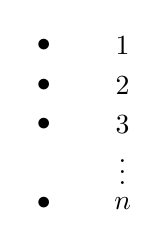
\begin{tikzpicture}[draw=white]	\draw (0,0) node{$\bullet$}-- ++(0,0.5) node{}-- ++(0,0.5) node{$\bullet$}-- ++(0,0.5) node{$\bullet$}-- ++(0,0.5) node{$\bullet$}; 
	\draw (1,0) node{$n$}-- ++(0,0.5) node{$\vdots$}-- ++(0,0.5) node{$3$}-- ++(0,0.5) node{$2$}-- ++(0,0.5) node{$1$}; 
	\end{tikzpicture}\]
	\item \textit{将所有点用一根连续的线连起来, 保证每个点都被线穿过.}
	\item \textit{列出所有不同的连接方式, 如果在两个图中, 对应的点与其周围的点的连接方式都相同, 那么这两个图等价.}
\end{enumerate}

第二个规则强制我们的图只能是完全连接的, 或者叫\emph{连通}的(linked), 也就是说, 它们连成一个整体. 如下的不连通图:
\begin{equation*}
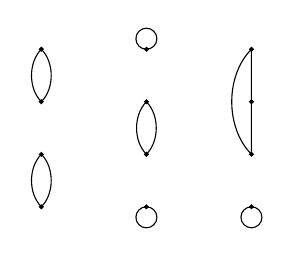
\begin{tikzpicture}[scale=.667]
\filldraw (0,0) circle(1pt) (2,0)circle (1pt) (4,0) circle(1pt)
          (0,1) circle(1pt) (2,1)circle (1pt) (4,1) circle(1pt)
          (0,2) circle(1pt) (2,2)circle (1pt) (4,2) circle(1pt)
          (0,3) circle(1pt) (2,3)circle (1pt) (4,3) circle(1pt);
\draw	  (0,0) .. controls (.25,.25)   and (.25,.75).. (0,1)
          (0,0) .. controls (-.25,.25)  and (-.25,.75).. (0,1)
		  (0,2) .. controls (.25,2.25)  and (.25,2.75).. (0,3)
		  (0,2) .. controls (-.25,2.25) and (-.25,2.75).. (0,3)
		  (2,3.2) circle(.2cm)
		  (2,2) .. controls+(.25,-.25) and (2.25,1.25)..(2,1)
		  (2,2) .. controls+(-.25,-.25)and (1.75,1.25)..(2,1)
		  (2,-.2) circle(.2cm)
		  (4,3) .. controls+(-.5,-.5) and +(-.5,.5)..(4,1)
		  (4,3) -- (4,1)
		  (4,-.2) circle(.2cm)
		  ;
\end{tikzpicture}
\end{equation*}
是不允许出现的. 第三个规则是说, 如果几个图(如下例)
\begin{equation*}
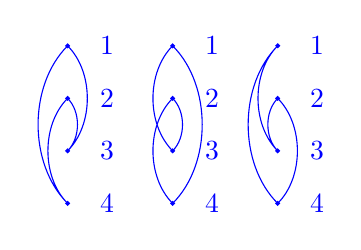
\begin{tikzpicture}[scale=.667,blue]
\filldraw (0,0) circle(1pt) (2,0)circle (1pt) (4,0) circle(1pt)
          (0,1) circle(1pt) (2,1)circle (1pt) (4,1) circle(1pt)
          (0,2) circle(1pt) (2,2)circle (1pt) (4,2) circle(1pt)
          (0,3) circle(1pt) (2,3)circle (1pt) (4,3) circle(1pt);
\draw	  (0,0) ..controls+(-.75,.75)   and +(-.75,-.75).. (0,3)
          (0,1) ..controls+(.5,.5)   and +(.5,-.5).. (0,3)
          (0,0) ..controls+(-.5,.5)   and +(-.5,-.5).. (0,2)
          (0,1) ..controls+(.25,.25) and +(.25,-.25).. (0,2)
          
          (2,0) ..controls+(.75,.75)and+(.75,-.75)..(2,3) 
          (2,1) ..controls+(-.5,.5)and+(-.5,-.5)..(2,3)
          (2,0) ..controls+(-.5,.5)and+(-.5,-.5)..(2,2)
          (2,1) ..controls+(.25,.25)and+(.25,-.25)..(2,2)
          
          (4,0) ..controls+(-.75,.75)and+(-.75,-.75)..(4,3)
          (4,1) ..controls+(-.5,.5)and+(-.5,-.5)..(4,3)
          (4,1) ..controls+(-.25,.25)and+(-.25,-.25)..(4,2) 
          (4,0) ..controls+(.5,.5)and+(.5,-.5)..(4,2)
;
\draw     (.75,0)node{4} (.75,1)node{3} (.75,2)node{2} (.75,3)node{1}
		  (2.75,0)node{4} (2.75,1)node{3} (2.75,2)node{2} (2.75,3)node{1}
		  (4.75,0)node{4} (4.75,1)node{3} (4.75,2)node{2} (4.75,3)node{1}
;
\end{tikzpicture}
\end{equation*}
以同一种方式连接,那么它们就等价: 1和3、4相连, 2和3、4相连, 3与1和2相连, 4与1和2相连. 为快速判断图之间是否等价, 可以将连线想象成粘在点上的橡皮筋, 我们可以任意拉扯伸缩这些皮筋. 如果两个图不等价 , 那么无论怎么对橡皮筋进行拉扯, 都不可能使两个图看起来一样. 因此:
\begin{equation*}
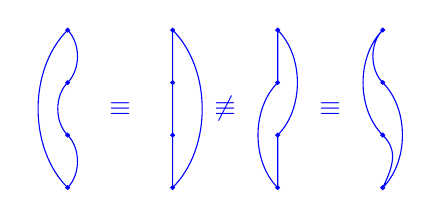
\begin{tikzpicture}[scale=.667,blue]
\filldraw (0,0) circle(1pt) (2,0)circle (1pt) (4,0) circle(1pt) (6,0) circle(1pt)
          (0,1) circle(1pt) (2,1)circle (1pt) (4,1) circle(1pt) (6,1) circle(1pt)
          (0,2) circle(1pt) (2,2)circle (1pt) (4,2) circle(1pt) (6,2) circle(1pt)
          (0,3) circle(1pt) (2,3)circle (1pt) (4,3) circle(1pt) (6,3) circle(1pt)
          ;
\draw	  (0,0) ..controls+(-.75,.75)   and +(-.75,-.75).. (0,3)
          (0,1) ..controls+(-.25,.25)   and +(-.25,-.25).. (0,2)
          (0,0) ..controls+(.25,.25)   and +(.25,-.25).. (0,1)
          (0,2) ..controls+(.25,.25) and +(.25,-.25).. (0,3)

          (2,0) -- (2,3) 
          (2,0) ..controls+(.75,.75)and+(.75,-.75)..(2,3)

          (4,0) -- (4,1)
          (4,1) ..controls+(.5,.5)and+(.5,-.5)..(4,3)
          (4,0) ..controls+(-.5,.5)and+(-.5,-.5)..(4,2) 
          (4,2) -- (4,3)
          
          (6,0)..controls+(.5,.5)and+(.5,-.5)..(6,2)
          (6,2)..controls+(-.25,.25)and+(-.25,-.25)..(6,3)
          (6,0)..controls+(.25,.5)and+(.25,-.25)..(6,1)
          (6,1)..controls+(-.5,.5)and+(-.5,-.5)..(6,3)
;
\draw     (1,1.5)node{$\equiv$} (3,1.5)node{$\not\equiv$} (5,1.5)node{$\equiv$};
\end{tikzpicture}
\end{equation*}
利用这些规则, 可以画出如下的图(至四阶):
\begin{equation*}
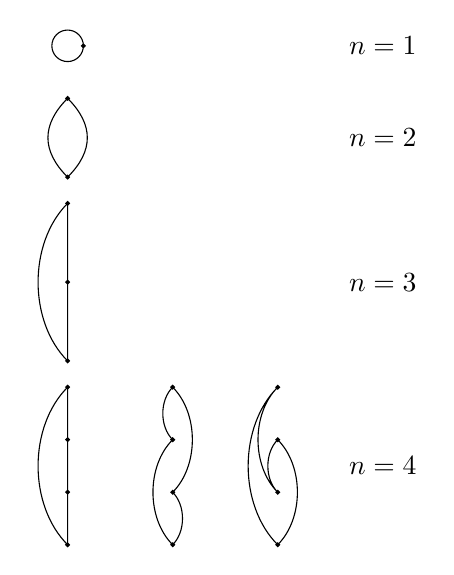
\begin{tikzpicture}[scale=.667]
\filldraw (0,0)circle(1pt) (0,1)circle(1pt) (0,2)circle(1pt) (0,3)circle(1pt)
          (0,3.5)circle(1pt) (0,5)circle(1pt) (0,6.5)circle(1pt)
          (0,7)circle(1pt) (0,8.5)circle(1pt)
          (.3,9.5)circle(1pt)
          
          (2,0)circle(1pt) (2,1)circle(1pt) (2,2)circle(1pt) (2,3)circle(1pt)
          
          (4,0)circle(1pt) (4,1)circle(1pt) (4,2)circle(1pt) (4,3)circle(1pt)
          ;
\draw     (0,0)..controls+(-.75,.75)and+(-.75,-.75)..(0,3)
          (0,0) -- (0,3)
          
          (0,3.5)..controls+(-.75,.75)and+(-.75,-.75)..(0,6.5)
          (0,3.5) -- (0,6.5)
          
          (0,7)..controls+(-.5,.5)and+(-.5,-.5)..(0,8.5)
          (0,7)..controls+(.5,.5)and+(.5,-.5)..(0,8.5)
          
          (0,9.5)circle(.3cm)
          
          (2,0)..controls+(-.5,.5)and+(-.5,-.5)..(2,2)
          (2,1)..controls+(.5,.5)and+(.5,-.5)..(2,3)
          (2,0)..controls+(.25,.25)and+(.25,-.25)..(2,1)
          (2,2)..controls+(-.25,.25)and+(-.25,-.25)..(2,3)
          
          (4,0)..controls+(.5,.5)and+(.5,-.5)..(4,2)
          (4,1)..controls+(-.25,.25)and+(-.25,-.25)..(4,2)
          (4,1)..controls+(-.5,.5)and+(-.5,-.5)..(4,3)
          (4,0)..controls+(-.75,.75)and+(-.75,-.75)..(4,3)
          ;
\draw     (6,1.5)node{$n=4$} (6,5)node{$n=3$} (6,7.75)node{$n=2$} (6,9.5)node{$n=1$};
\end{tikzpicture}
\end{equation*}
读者通过尝试应当可以使自己确信, 以上就是所有可能的相异图(直到四阶). 现在给连线加上箭头, 注意要保证每个点都有线穿入和穿出. 若以1来标记向下的线, 2来标记向上的线, 则有两种标法:
\begin{equation*}
\begin{tikzpicture}
\filldraw (0,0)circle(1pt) (0,-.75)circle(1pt) (0,.75)circle(1pt);
\draw     (0,-.75)..controls+(-.45,.45)and+(-.45,-.45)..(0,.75)
          (0,-.75)--(0,.75);
\draw[arrows = {-Latex[width=0pt 5, length=5pt]}] (.3,.15)--(2.2,1.1);
\draw[arrows = {-Latex[width=0pt 5, length=5pt]}] (.3,-.15)--(2.2,-1.1);
\begin{scope}[decoration = {markings, mark= at position 0.54 with {\arrow{latex}}} ]
\filldraw (3,.5) circle(1pt) (3,1.25)circle(1pt) (3,2)circle(1pt)
          (3,-.5)circle(1pt) (3,-1.25)circle(1pt) (3,-2)circle(1pt);
\draw[postaction={decorate}]     (3,.5)..controls+(-.5,.45)and+(-.5,-.45)..node[left]{2}(3,2);
\draw[postaction={decorate}]     (3,2)--node[right]{1}(3,1.25);
\draw[postaction={decorate}]     (3,1.25)--node[right]{1}(3,.5);
\draw[postaction={decorate}]     (3,-.5)..controls+(-.45,-.45)and+(-.45,.45)..node[left]{1}(3,-2);
\draw[postaction={decorate}]     (3,-2)--node[right]{2}(3,-1.25);
\draw[postaction={decorate}]     (3,-1.25)--node[right]{2}(3,-.5);
\end{scope}
\end{tikzpicture}
\end{equation*}
当$n=1$时, 会有一个小问题, 图上的箭头在某部分是向上的, 在另一部分是向下的
\begin{equation*}
\begin{tikzpicture}[scale=1]
\begin{scope}[decoration = {markings, mark= {between positions 0 and 1 step .35 with {
			\draw[arrows = {-Latex[width=0pt 5, length=5pt]}] (0pt,.1pt) -- (1pt,0pt);}}} ]
\draw[postaction={decorate}] (0.25,0.43301270189221932338186158537647) arc [start angle=60, end angle=420, radius=.5];
\filldraw (.5,0)circle(1pt);
\end{scope}
\end{tikzpicture}
\end{equation*}
我们可以将圆圈定义为空穴线来规避这个问题. 按照以上的办法, 我们总共可以画出如下这么多的图:
\begin{equation*}
\diagsize
\begin{tikzpicture}[scale=.667]
\filldraw    (0,0)circle(1pt) (0,1)circle(1pt) (0,2)circle(1pt) (0,3)circle(1pt)
             (1.5,0)circle(1pt) (1.5,1)circle(1pt) (1.5,2)circle(1pt) (1.5,3)circle(1pt)
             (3,0)circle(1pt) (3,1)circle(1pt) (3,2)circle(1pt) (3,3)circle(1pt)
             (4.5,0)circle(1pt) (4.5,1)circle(1pt) (4.5,2)circle(1pt) (4.5,3)circle(1pt)
             (6,0)circle(1pt) (6,1)circle(1pt) (6,2)circle(1pt) (6,3)circle(1pt)
             (7.5,0)circle(1pt) (7.5,1)circle(1pt) (7.5,2)circle(1pt) (7.5,3)circle(1pt)
             (0,3.5)circle(1pt) (0,5)circle(1pt) (0,6.5)circle(1pt) 
             (2,3.5)circle(1pt) (2,5)circle(1pt) (2,6.5)circle(1pt) 
             (0,7)circle(1pt) (0,8.5)circle(1pt)
             (.3,9.5)circle(1pt)
;
\begin{scope}% line between dots
\draw[blue] (0,9.5)circle(.3cm); % the circle
\path [draw=blue,postaction={on each segment={mid arrow}}]
(0,8.5)..controls+(-.45,-.45)and+(-.45,.45)..(0,7) % n = 2, 1st diagram
(0,7)..controls+(.45,.45)and+(.45,-.45)..(0,8.5)   %
%=======================================================
(0,6.5)..controls+(-.75,-.75)and+(-.75,.75)..node[left]{1}(0,3.5) % n=3, 1st
(0,3.5) -- node[right]{2}(0,5)--node[right]{2}(0,6.5)
(2,3.5)..controls+(-.75,.75)and+(-.75,-.75)..node[left]{2}(2,6.5) % n=3, 2st
(2,6.5) -- node[right]{1}(2,5)--node[right]{1}(2,3.5)
%=======================================================
(0,0)..controls+(.25,.25)and+(.25,-.25)..node[right]{2}(0,1) % n=4, 1st
(0,1)..controls+(.5,.5)and+(.5,-.5)..node[right]{2}(0,3)
(0,3)..controls+(-.25,-.25)and+(-.25,.25)..node[left]{1}(0,2)
(0,2)..controls+(-.5,-.5)and+(-.5,.5)..node[left]{1}(0,0)
(1.5,1)..controls+(.25,-.25)and+(.25,.25)..node[right]{1}(1.5,0) % n=4, 2nd
(1.5,3)..controls+(.5,-.5)and+(.5,.5)..node[right]{1}(1.5,1)
(1.5,2)..controls+(-.25,.25)and+(-.25,-.25)..node[left]{2}(1.5,3)
(1.5,0)..controls+(-.5,.5)and+(-.5,-.5)..node[left]{2}(1.5,2)
(3,0)--node[right]{2}(3,1)--node[right]{2}(3,2)--node[right]{2}(3,3) % n=4, 3rd
(3,3)..controls+(-.75,-.75)and+(-.75,.75)..node[left]{1}(3,0)
(4.5,3)--node[right]{1}(4.5,2)--node[right]{1}(4.5,1)--node[right]{1}(4.5,0) % n=4, 4th
(4.5,0)..controls+(-.75,.75)and+(-.75,-.75)..node[left]{2}(4.5,3)
(6,0)..controls+(.5,.5)and+(.5,-.5)..node[left]{1}(6,2) % n=4, 5th
(6,2)..controls+(.25,-.25)and+(.25,.25)..node[left]{1}(6,1)
(6,1)..controls+(-.5,.5)and+(-.5,-.5)..node[right]{2}(6,3)
(6,3)..controls+(-.75,-.75)and+(-.75,.75)..node[left]{1}(6,0)
(7.5,2)..controls+(.5,-.5)and+(.5,.5)..node[left]{2}(7.5,0) % n=4, 6th
(7.5,1)..controls+(.25,.25)and+(.25,-.25)..node[left]{2}(7.5,2)
(7.5,3)..controls+(-.5,-.5)and+(-.5,.5)..node[right]{1}(7.5,1)
(7.5,0)..controls+(-.75,.75)and+(-.75,-.75)..node[left]{2}(7.5,3)
;
\end{scope}
\normalsize
\draw     (9,1.5)node{$n=4$} (9,5)node{$n=3$} (9,7.75)node{$n=2$} (9,9.5)node{$n=1$};
\end{tikzpicture}
\end{equation*}

现\emph{假设}所有$n$个点的图和所有$n$阶能量项之间存在一一映射, 此处我们给出由图到能量项的表达式的转换规则. 存在这种对应关系是很奇妙的一件事. 转换规则如下:
\begin{enumerate}
	\item 每个点为分母贡献一个因子$\braket{\textit{穿入线的标号}|\vs|\textit{穿出线的标号}}$.
	\item 每一对相邻点贡献一个分母上的因子\[ \sum E_\mathrm{空穴}-\sum E^{(0)}_\mathrm{粒子}\]
	其中求和遍及所有与两个点之间的一条水平线相交的空穴线和粒子线.
	\item 表达式的正负号为$(-)^{h+l}$, $h$是空穴线的数目, $l$是闭合圈图的数目. 本节的图中$l$总是1, 这里给出更一般的规则以利后用.
\end{enumerate}
这个规则很容易运用. 考虑四阶图
\begin{equation*}
\begin{tikzpicture}
\diagsize
\filldraw[blue] 
(0,0)circle(1pt) (0,1)circle(1pt) (0,2)circle(1pt) (0,3)circle(1pt);
\draw[dashed] (-2,.5)node[left]{$C$}--(2,.5)
              (-2,1.3)node[left]{$B$}--(2,1.3)
              (-2,2.5)node[left]{$A$}--(2,2.5);
\begin{scope}
\path [draw=blue,postaction={on each segment={mid arrow}}]
(0,0)..controls+(.5,.5)and+(.5,-.5)..node[left]{1}(0,2) % n=4, 5th
(0,2)..controls+(.25,-.25)and+(.25,.25)..node[left]{1}(0,1)
(0,1)..controls+(-.5,.5)and+(-.5,-.5)..node[right]{2}(0,3)
(0,3)..controls+(-.75,-.75)and+(-.75,.75)..node[left]{1}(0,0);
\end{scope}
\end{tikzpicture}
\end{equation*}
最上面的两个点每个为分母贡献一个因子$\braket{2|\vs|1}=V_{21}$, 剩余的点每个贡献$\braket{1|\vs|2}=V_{12}$. 虚线$A,C$每个都为分母贡献一因子$E_1^{(0)} - E_2^{(0)}$, 虚线$B$贡献一个因子$(2E_1^{(0)} - 2E_2^{(0)})$. 此外, 该图有2个空穴线($h=2$)1个闭合圈图($l=1$), 所以要将式子乘以$(-1)^3$. 所以最终有
\begin{equation*}
\begin{tikzpicture}[baseline={(current bounding box.center)}, scale=1]
\diagsize
\filldraw[blue] 
(0,0)circle(1pt) (0,1)circle(1pt) (0,2)circle(1pt) (0,3)circle(1pt);
\begin{scope}
\path [draw=blue,postaction={on each segment={mid arrow}}]
(0,0)..controls+(.5,.5)and+(.5,-.5)..node[left]{1}(0,2) % n=4, 5th
(0,2)..controls+(.25,-.25)and+(.25,.25)..node[left]{1}(0,1)
(0,1)..controls+(-.5,.5)and+(-.5,-.5)..node[right]{2}(0,3)
(0,3)..controls+(-.75,-.75)and+(-.75,.75)..node[left]{1}(0,0);
\end{scope}
\end{tikzpicture} = (-)^3\frac{(V_{12}V_{21})^2}{\left(E_1^{(0)} - E_2^{(0)}\right)\left(2E_1^{(0)} - 2E_2^{(0)}\right)} = \frac{(V_{12}V_{21})^2}{2\left(E_1^{(0)} - E_2^{(0)}\right)^2} 
\end{equation*}

值得注意, 在我们的在转化规则下, 如下的每一对图都给出相同结果
\begin{align*}
%\tikzset{scale=.67}
\begin{tikzpicture}[baseline={(current bounding box.center)},scale=.67]\diagsize
\filldraw[blue] 
(4.5,0)circle(1pt) (4.5,1)circle(1pt) (4.5,2)circle(1pt) (4.5,3)circle(1pt); 
\path [draw=blue,postaction={on each segment={mid arrow}}] (4.5,3)--node[right]{1}(4.5,2)--node[right]{1}(4.5,1)--node[right]{1}(4.5,0) % n=4, 4th
(4.5,0)..controls+(-.75,.75)and+(-.75,-.75)..node[left]{2}(4.5,3);
\end{tikzpicture} \hspace{.5cm}
 &\equiv \hspace{.5cm}
\begin{tikzpicture}[baseline={(current bounding box.center)},scale=.67]
	\filldraw[blue] 
(4.50,0)circle(1pt)   (4.5,3)circle(1pt); 
\path [draw=blue,postaction={on each segment={mid arrow}}] (4.5,3) arc (45:15:2.12cm)node[right,midway]{1} node{\tikz{\filldraw[blue](0,0)circle(1pt)}} arc (15:-15:2.12cm)node[right,midway]{1}node{\tikz{\filldraw[blue](0,0)circle(1pt)}} arc (-15:-45:2.12cm)
(4.5,0) arc(225:135:2.12cm)node[left,midway]{2};
\end{tikzpicture}\vspace{.5cm}\\
\begin{tikzpicture}[baseline={(current bounding box.center)},scale=.67]\diagsize
\filldraw[blue] 
(0,0)circle(1pt) (0,1)circle(1pt) (0,2)circle(1pt) (0,3)circle(1pt); 
\path [draw=blue,postaction={on each segment={mid arrow}}] (0,0)..controls+(.25,.25)and+(.25,-.25)..node[right]{2}(0,1) % n=4, 1st
(0,1)..controls+(.5,.5)and+(.5,-.5)..node[right]{2}(0,3)
(0,3)..controls+(-.25,-.25)and+(-.25,.25)..node[left]{1}(0,2)
(0,2)..controls+(-.5,-.5)and+(-.5,.5)..node[left]{1}(0,0);
\end{tikzpicture} \hspace{.5cm}
&\equiv \hspace{.5cm}
\begin{tikzpicture}[baseline={(current bounding box.center)},scale=.67]\diagsize
\filldraw[blue] 
(4.50,0)circle(1pt)   (4.5,3)circle(1pt); 
\path [draw=blue,postaction={on each segment={mid arrow}}] (4.5,0) arc (-45:-15:2.12cm)node[right,midway]{2} node{\tikz{\filldraw[blue](0,0)circle(1pt)}} arc (-15:45:2.12cm)node[right,midway]{2}node{\tikz{\filldraw[blue](0,0)circle(1pt)}}
(4.5,3) arc(135:165:2.12cm)node[left,midway]{1} arc(165:225:2.12cm)node[midway,left]{1};
\end{tikzpicture}\vspace{.5cm}\\
\begin{tikzpicture}[baseline={(current bounding box.center)},scale=.67]\diagsize
\filldraw[blue] 
(6,0)circle(1pt) (6,1)circle(1pt) (6,2)circle(1pt) (6,3)circle(1pt); 
\path [draw=blue,postaction={on each segment={mid arrow}}] 
(6,0)..controls+(.5,.5)and+(.5,-.5)..node[left]{1}(6,2) % n=4, 5th
(6,2)..controls+(.25,-.25)and+(.25,.25)..node[left]{1}(6,1)
(6,1)..controls+(-.5,.5)and+(-.5,-.5)..node[right]{2}(6,3)
(6,3)..controls+(-.75,-.75)and+(-.75,.75)..node[left]{1}(6,0);
\end{tikzpicture} \hspace{.5cm}
&\equiv \hspace{.5cm}
\begin{tikzpicture}[baseline={(current bounding box.center)},scale=.67]\diagsize
\path [draw=blue,postaction={on each segment={mid arrow}}] 
(6,0)arc(290:365:1.58cm)node[right,midway]{2}node{\tikz{\filldraw[blue](0,0)circle(1pt)}} arc (90:160:1) node[above,pos=.5]{1}node{\tikz{\filldraw[blue](0,0)circle(1pt)}} arc(-15:45:1.58)node[right,pos=.6]{2}node{\tikz{\filldraw[blue](0,0)circle(1pt)}} to [bend right] node[left,midway]{1}node[pos=1]{\tikz{\filldraw[blue](0,0)circle(1pt)}}(6,0) ;
\end{tikzpicture}
\end{align*}
这事实告诉我们, 画图时不必将各点严格按照竖线排列. 实际上, \emph{在不改变各点竖直顺序的前提下, 我们可以对图进行任意扭动}.

表6.1中按照之前的规则计算出了所有的二、三、四阶图对应的代数式. 按习惯, 一阶泡泡图定为
\begin{equation*}
\begin{tikzpicture}[baseline={(current bounding box.center)},scale=1]
\begin{scope}[blue, decoration = {markings, mark= {between positions 0 and 1 step .35 with {
			\draw[arrows = {-Latex[width=0pt 5, length=5pt]}] (0pt,.1pt) -- (1pt,0pt);}}} ]
\draw[postaction={decorate}] (0.25,0.43301270189221932338186158537647) arc [start angle=60, end angle=420, radius=.5];
\filldraw (.5,0)circle(1pt);
\end{scope}
\end{tikzpicture} = V_{11}
\end{equation*}
检视表6.1可以发现, 按照我们的规则把图换成算式, 然后将各阶图对应的算式加起来, 就得到该阶的能量修正, 其结果和上一节所得的完全相同. 
\exercise{写出虚线仅会穿过一条空穴线和一条粒子线的五阶图, 求出对应的算式并证明这些图之和对应着
\[
\frac{V_{12}V_{21}(V_{22}-V_{11})^3}{(E_1^{(0)}-E_2^{(0)})^4}
\]
\textit{提示}: 这样的图共有八个. 你可以把三个点加在二阶图上来生成所有可能的五阶图.
}
\begin{table}[H]
	\caption{图到公式的转换}
	\begin{tabularx}{\textwidth}{cY}\hline
	\begin{tikzpicture}[baseline={(current bounding box.center)},scale=.6]  
	\path [draw=blue,postaction={on each segment={mid arrow}}] 
	(4.5,0) node{\tikz{\filldraw[blue](0,0)circle(1pt)}}
	arc (-45:45:2.12cm)node[right,midway]{2} node{\tikz{\filldraw[blue](0,0)circle(1pt)}} arc(135:225:2.12cm)node[left,midway]{1};
	\end{tikzpicture} & $(-)^{1+1}\dfrac{\braket{1|\vs|2}\braket{2|\vs|1}}{E_1^{(0)}-E_2^{(0)}}=\dfrac{V_{12}V_{21}}{E_1^{(0)}-E_2^{(0)}}$ \\\hline
	\begin{tikzpicture}[baseline={(current bounding box.center)},scale=.6] 
	\path [draw=blue,postaction={on each segment={mid arrow}}] 
	(4.5,0) node{\tikz{\filldraw[blue](0,0)circle(1pt)}}
	arc (-45:0:2.12cm)node[right,midway]{2} node{\tikz{\filldraw[blue](0,0)circle(1pt)}}
	arc (0:45:2.12cm)node[right,midway]{2} node{\tikz{\filldraw[blue](0,0)circle(1pt)}} 
	arc (135:225:2.12cm)node[left,midway]{1};
	\end{tikzpicture} & 
	$(-)^{1+1}\dfrac{\braket{1|\vs|2}\braket{2|\vs|2}\braket{2|\vs|1}}{(E_1^{(0)}-E_2^{(0)})^2}=\dfrac{V_{12}V_{22}V_{21}}{(E_1^{(0)}-E_2^{(0)})^2}$ \\\hline
	\begin{tikzpicture}[baseline={(current bounding box.center)},scale=.6] 
	\path [draw=blue,postaction={on each segment={mid arrow}}] 
	(4.5,0) node{\tikz{\filldraw[blue](0,0)circle(1pt)}}
	arc (225:135:2.12cm)node[left,midway]{2} node{\tikz{\filldraw[blue](0,0)circle(1pt)}}
	arc (45:0:2.12cm)node[right,midway]{1} node{\tikz{\filldraw[blue](0,0)circle(1pt)}} 
	arc (0:-45:2.12cm)node[left,midway]{1};
	\end{tikzpicture} & $(-)^{2+1}\dfrac{\braket{1|\vs|2}\braket{2|\vs|1}\braket{1|\vs|1}}{(E_1^{(0)}-E_2^{(0)})^2}=\dfrac{V_{12}V_{21}V_{11}}{(E_1^{(0)}-E_2^{(0)})^2}$\\\hline
	\begin{tikzpicture}[baseline={(current bounding box.center)},scale=.6]  
	\path [draw=blue,postaction={on each segment={mid arrow}}] 
	(4.5,0) node{\tikz{\filldraw[blue](0,0)circle(1pt)}}
	arc (-45:45:2.12cm)node[right,midway]{2} node{\tikz{\filldraw[blue](0,0)circle(1pt)}} arc(135:165:2.12cm)node[left,midway]{1} node{\tikz{\filldraw[blue](0,0)circle(1pt)}}
	arc(165:195:2.12cm)node[left,midway]{1} node{\tikz{\filldraw[blue](0,0)circle(1pt)}}
	arc(195:225:2.12cm)node[left,midway]{1} node{\tikz{\filldraw[blue](0,0)circle(1pt)}};
	\end{tikzpicture} 
	& $(-)^{3+1}\dfrac{\braket{1|\vs|2}\braket{2|\vs|1}\braket{1|\vs|1}\braket{1|\vs|1}}{(E_1^{(0)}-E_2^{(0)})^3}=\dfrac{V_{12}V_{21}V_{11}^2}{(E_1^{(0)}-E_2^{(0)})^3}$ \\\hline
	\begin{tikzpicture}[baseline={(current bounding box.center)},scale=.6] 
	\path [draw=blue,postaction={on each segment={mid arrow}}] 
	(4.5,0) node{\tikz{\filldraw[blue](0,0)circle(1pt)}}
	arc (-45:-15:2.12cm)node[right,midway]{2} node{\tikz{\filldraw[blue](0,0)circle(1pt)}}
	arc (-15:45:2.12cm)node[right,midway]{2} node{\tikz{\filldraw[blue](0,0)circle(1pt)}} 
	arc (135:165:2.12cm)node[left,midway]{1} node{\tikz{\filldraw[blue](0,0)circle(1pt)}} 
	arc (165:225:2.12cm)node[left,midway]{1} node{\tikz{\filldraw[blue](0,0)circle(1pt)}} ;
	\end{tikzpicture} & 
	$(-)^{2+1}\dfrac{\braket{1|\vs|2}\braket{2|\vs|2}\braket{2|\vs|1}\braket{1|\vs|1}}{(E_1^{(0)}-E_2^{(0)})^3}=\dfrac{V_{12}V_{22}V_{21}V_{11}}{(E_1^{(0)}-E_2^{(0)})^3}$ \\\hline
	\begin{tikzpicture}[baseline={(current bounding box.center)},scale=.6] 
	\path [draw=blue,postaction={on each segment={mid arrow}}] 
	(4.5,0) node{\tikz{\filldraw[blue](0,0)circle(1pt)}}
	arc (225:165:2.12cm)node[right,midway]{2} node{\tikz{\filldraw[blue](0,0)circle(1pt)}}
	arc (165:135:2.12cm)node[right,midway]{2} node{\tikz{\filldraw[blue](0,0)circle(1pt)}} 
	arc (45:-15:2.12cm)node[left,midway]{1} node{\tikz{\filldraw[blue](0,0)circle(1pt)}} 
	arc (-15:-45:2.12cm)node[left,midway]{1} node{\tikz{\filldraw[blue](0,0)circle(1pt)}} ;
	\end{tikzpicture} & 
	$(-)^{2+1}\dfrac{\braket{1|\vs|2}\braket{2|\vs|2}\braket{2|\vs|1}\braket{1|\vs|1}}{(E_1^{(0)}-E_2^{(0)})^3}=\dfrac{V_{12}V_{22}V_{21}V_{11}}{(E_1^{(0)}-E_2^{(0)})^3}$ \\\hline
	\begin{tikzpicture}[baseline={(current bounding box.center)},scale=.6] 
	\path [draw=blue,postaction={on each segment={mid arrow}}] 
	(4.5,0) node{\tikz{\filldraw[blue](0,0)circle(1pt)}}
	arc (225:195:2.12cm)node[left,midway]{2} node{\tikz{\filldraw[blue](0,0)circle(1pt)}}
	arc (195:165:2.12cm)node[left,midway]{2} node{\tikz{\filldraw[blue](0,0)circle(1pt)}} 
	arc (165:135:2.12cm)node[left,midway]{2} node{\tikz{\filldraw[blue](0,0)circle(1pt)}} 
	arc (45:-45:2.12cm)node[right,midway]{1} node{\tikz{\filldraw[blue](0,0)circle(1pt)}} ;
	\end{tikzpicture} & 
	$(-)^{1+1}\dfrac{\braket{1|\vs|2}\braket{2|\vs|2}\braket{2|\vs|2}\braket{1|\vs|1}}{(E_1^{(0)}-E_2^{(0)})^3}=\dfrac{V_{12}V_{22}^2V_{21}}{(E_1^{(0)}-E_2^{(0)})^3}$ \\\hline
	\begin{tikzpicture}[baseline={(current bounding box.center)},scale=.6]
	\path [draw=blue,postaction={on each segment={mid arrow}}] 
	(6,0) to [bend right] node[right,midway]{2} node[pos=0]{\dian}
	(7,2) to [bend right] node[above,midway]{1} node[pos=0]{\dian}
	(6,1) to [bend right] node[right,midway]{2} node[pos=0]{\dian}
	(5,2.8) to [bend right] node[left,midway]{1} node[pos=0]{\dian}
	(6,0) ;
	\end{tikzpicture} & $(-)^{2+1}\dfrac{\braket{1|\vs|2}\braket{2|\vs|1}\braket{1|\vs|2}\braket{2|\vs|1}}{(E_1^{(0)}-E_2^{(0)})^2(2E_1^{(0)} - 2E_2^{(0)})}=\dfrac{(V_{12}V_{21})^2}{2(E_1^{(0)}-E_2^{(0)})^3}$\\\hline
	\begin{tikzpicture}[baseline={(current bounding box.center)},scale=.6]
	\path [draw=blue,postaction={on each segment={mid arrow}}] 
	(6,0) to [bend left] node[left,midway]{2} node[pos=0]{\dian}
	(5,3) to [bend left] node[right,midway]{1} node[pos=0]{\dian}
	(6,1) to [bend left] node[above,midway]{2} node[pos=0]{\dian}
	(7,1.8) to [bend left] node[right,midway]{1} node[pos=0]{\dian}
	(6,0);
	\end{tikzpicture} & $(-)^{2+1}\dfrac{\braket{1|\vs|2}\braket{2|\vs|1}\braket{1|\vs|2}\braket{2|\vs|1}}{(E_1^{(0)}-E_2^{(0)})^2(2E_1^{(0)} - 2E_2^{(0)})}=\dfrac{(V_{12}V_{21})^2}{2(E_1^{(0)}-E_2^{(0)})^3}$\\\hline
	\end{tabularx}
\label{t6.1}
\end{table}

\subsection{$N$个态的图微扰论}
本节将之前所发展的RS微扰论的图表示应用到$N$-态系统上. 考虑如何找到这样一个系统最低本征值的微扰展开. 现下我们仍然只有一个空穴态$\ket{1}$, 但有$N-1$个粒子态$\ket{n}, n=2,3,\cdots,N$. 我们仍然按照之前的办法来画图, 但要注意现在粒子线的标签可以式任意的$n$. 举个例子, 下图
\begin{equation*}
	\begin{tikzpicture}[baseline={(current bounding box.center)},scale=.6] 
\path [draw=blue,postaction={on each segment={mid arrow}}] 
(4.5,0) node{\tikz{\filldraw[blue](0,0)circle(1pt)}}
arc (225:180:2.12cm) node{\tikz{\filldraw[blue](0,0)circle(1pt)}}
arc (180:135:2.12cm) node{\tikz{\filldraw[blue](0,0)circle(1pt)}} 
arc (45:-45:2.12cm) node{\tikz{\filldraw[blue](0,0)circle(1pt)}} ;
\end{tikzpicture}
\end{equation*}
可以按不同的方式来标记:
\begin{equation*}
\begin{tikzpicture}[baseline={(current bounding box.center)},scale=.6] 
\path [draw=blue,postaction={on each segment={mid arrow}}] 
(4.5,0) node{\tikz{\filldraw[blue](0,0)circle(1pt)}}
arc (225:180:2.12cm) node[left,midway]{2} node{\tikz{\filldraw[blue](0,0)circle(1pt)}}
arc (180:135:2.12cm) node[left,midway]{2} node{\tikz{\filldraw[blue](0,0)circle(1pt)}} 
arc (45:-45:2.12cm) node[right,midway]{1} node{\tikz{\filldraw[blue](0,0)circle(1pt)}} ;
\end{tikzpicture}
\begin{tikzpicture}[baseline={(current bounding box.center)},scale=.6] 
\path [draw=blue,postaction={on each segment={mid arrow}}] 
(4.5,0) node{\tikz{\filldraw[blue](0,0)circle(1pt)}}
arc (225:180:2.12cm) node[left,midway]{3} node{\tikz{\filldraw[blue](0,0)circle(1pt)}}
arc (180:135:2.12cm) node[left,midway]{2} node{\tikz{\filldraw[blue](0,0)circle(1pt)}} 
arc (45:-45:2.12cm)  node[right,midway]{1} node{\tikz{\filldraw[blue](0,0)circle(1pt)}} ;
\end{tikzpicture}
\begin{tikzpicture}[baseline={(current bounding box.center)},scale=.6] 
\path [draw=blue,postaction={on each segment={mid arrow}}] 
(4.5,0) node{\tikz{\filldraw[blue](0,0)circle(1pt)}}
arc (225:180:2.12cm) node[left,midway]{3}  node{\tikz{\filldraw[blue](0,0)circle(1pt)}}
arc (180:135:2.12cm) node[left,midway]{3}  node{\tikz{\filldraw[blue](0,0)circle(1pt)}} 
arc (45:-45:2.12cm)  node[right,midway]{1} node{\tikz{\filldraw[blue](0,0)circle(1pt)}} ;
\end{tikzpicture}
\begin{tikzpicture}[baseline={(current bounding box.center)},scale=.6] 
\path [draw=blue,postaction={on each segment={mid arrow}}] 
(4.5,0) node{\tikz{\filldraw[blue](0,0)circle(1pt)}}
arc (225:180:2.12cm) node[left,midway]{4} node{\tikz{\filldraw[blue](0,0)circle(1pt)}}
arc (180:135:2.12cm) node[left,midway]{3} node{\tikz{\filldraw[blue](0,0)circle(1pt)}} 
arc (45:-45:2.12cm)  node[right,midway]{1}node{\tikz{\filldraw[blue](0,0)circle(1pt)}} ;
\end{tikzpicture}
\begin{tikzpicture}[baseline={(current bounding box.center)},scale=.6] 
\path [draw=blue,postaction={on each segment={mid arrow}}] 
(4.5,0) node{\tikz{\filldraw[blue](0,0)circle(1pt)}}
arc (225:180:2.12cm) node[left,midway]{4}  node{\tikz{\filldraw[blue](0,0)circle(1pt)}}
arc (180:135:2.12cm) node[left,midway]{2}  node{\tikz{\filldraw[blue](0,0)circle(1pt)}} 
arc (45:-45:2.12cm)  node[right,midway]{1} node{\tikz{\filldraw[blue](0,0)circle(1pt)}} ;
\end{tikzpicture}
\end{equation*}
等等. 一般地我们可以写出
\begin{equation*}
\begin{tikzpicture}[baseline={(current bounding box.center)},scale=.6] 
\path [draw=blue,postaction={on each segment={mid arrow}}] 
(4.5,0) node{\tikz{\filldraw[blue](0,0)circle(1pt)}}
arc (225:180:2.12cm) node[left,midway]{$m$}  node{\tikz{\filldraw[blue](0,0)circle(1pt)}}
arc (180:135:2.12cm) node[left,midway]{$n$}  node{\tikz{\filldraw[blue](0,0)circle(1pt)}} 
arc (45:-45:2.12cm)  node[right,midway]{1} node{\tikz{\filldraw[blue](0,0)circle(1pt)}} ;
\end{tikzpicture}
\end{equation*}
其中的标号$m,n$可以独立地取$2$到$N$的任何值. 其中一类图如下
\begin{equation*}
\begin{tikzpicture}[baseline={(current bounding box.center)},scale=.6] 
\path [draw=blue,postaction={on each segment={mid arrow}}] 
(4.5,0) node{\tikz{\filldraw[blue](0,0)circle(1pt)}}
arc (225:180:2.12cm) node[left,midway]{$n$}  node{\tikz{\filldraw[blue](0,0)circle(1pt)}}
arc (180:135:2.12cm) node[left,midway]{$n$}  node{\tikz{\filldraw[blue](0,0)circle(1pt)}} 
arc (45:-45:2.12cm)  node[right,midway]{1} node{\tikz{\filldraw[blue](0,0)circle(1pt)}} ;
\end{tikzpicture}
\end{equation*}
我们称这样的图为\emph{对角的}. 为得到这些推广了的图的数学表达式, 我们需要在之前的规则上增加一条:
\begin{itemize}\itshape
	\item[4] 求和时要对所有粒子标签求和. 
\end{itemize}

这里来看一个示例. 计算二阶和三阶能量
\begin{subequations}
\begin{align}
	\begin{tikzpicture}[baseline={(current bounding box.center)},scale=.6] 
		\path [draw=blue,postaction={on each segment={mid arrow}}] 
		(4.5,0) node{\tikz{\filldraw[blue](0,0)circle(1pt)}}
		arc (-45:45:2.12cm) node[right,midway]{$n$} node{\tikz{\filldraw[blue](0,0)circle(1pt)}}
		arc (135:225:2.12cm)node[left,midway]{1}  node{\tikz{\filldraw[blue](0,0)circle(1pt)}};
	\end{tikzpicture} & = \sum_{n\neq 1}\frac{V_{1n}V_{n1}}{E_1^{(0)} - E_n^{(0)}} = \sum_n'\frac{V_{1n}V_{n1}}{E_1^{(0)} - E_n^{(0)}}\\
	\begin{tikzpicture}[baseline={(current bounding box.center)},scale=.6] 
\path [draw=blue,postaction={on each segment={mid arrow}}] 
(4.5,0) node{\tikz{\filldraw[blue](0,0)circle(1pt)}}
arc (225:180:2.12cm) node[left,midway]{$m$}  node{\tikz{\filldraw[blue](0,0)circle(1pt)}}
arc (180:135:2.12cm) node[left,midway]{$n$}  node{\tikz{\filldraw[blue](0,0)circle(1pt)}} 
arc (45:-45:2.12cm)node[right,midway]{1}  node{\tikz{\filldraw[blue](0,0)circle(1pt)}};
\end{tikzpicture} 
+
\begin{tikzpicture}[baseline={(current bounding box.center)},scale=.6] 
\path [draw=blue,postaction={on each segment={mid arrow}}] 
(4.5,0) node{\tikz{\filldraw[blue](0,0)circle(1pt)}}
arc (-45:45:2.12cm) node[right,midway]{$n$} node{\tikz{\filldraw[blue](0,0)circle(1pt)}}
arc (135:180:2.12cm)node[left,midway]{1}  node{\tikz{\filldraw[blue](0,0)circle(1pt)}}
arc (180:225:2.12cm)node[left,midway]{1}  node{\tikz{\filldraw[blue](0,0)circle(1pt)}};
\end{tikzpicture} 
& = \sum_{n\neq 1}\frac{V_{1n}V_{n1}}{E_1^{(0)} - E_n^{(0)}} = \sum_n'\frac{V_{1n}V_{n1}}{E_1^{(0)} - E_n^{(0)}}
\end{align}
\end{subequations}
这两个表达式与之前所得到的二阶、三阶能量的表达式(6.12)(6.15)在$i=1$的情况完全相同. 如果现在要得到某个态$i$的微扰表达式, 而且$i$不一定是最低能态, 我们要如何处理? 图的形状怎么样呢? 我们很容易能够验证, 如果将空穴线标为$i$, 粒子线标为$m,n,k$, 其取值为$1,2,\ldots,i-1$和$i+1,\ldots,N$, 那么答案就与之前的相同. 那么现在我们对RS微扰论就有了一个完整的图表示框架, 可以将其应该用于任意的微扰和任意的零阶态上.
\exercise{
使用图技术得到一个$N$-态系统中特定态的四阶微扰能(比如态$i$). 也就是, 计算如下图的表达式:
\begin{equation*}
\begin{tikzpicture}[baseline={(current bounding box.center)},scale=.6] 
\path [draw=blue,postaction={on each segment={mid arrow}}] 
(4.5,0) node{\tikz{\filldraw[blue](0,0)circle(1pt)}}
arc (225:195:2.12cm) node[left,midway]{$m$} node{\tikz{\filldraw[blue](0,0)circle(1pt)}}
arc (195:165:2.12cm) node[left,midway]{$n$} node{\tikz{\filldraw[blue](0,0)circle(1pt)}}
arc (165:135:2.12cm) node[left,midway]{$k$} node{\tikz{\filldraw[blue](0,0)circle(1pt)}}

arc (45:-45:2.12cm) node[right,midway]{$i$} node{\tikz{\filldraw[blue](0,0)circle(1pt)}} ;
\end{tikzpicture}
\begin{tikzpicture}[baseline={(current bounding box.center)},scale=.6] 
\path [draw=blue,postaction={on each segment={mid arrow}}] 
(4.5,0) node{\tikz{\filldraw[blue](0,0)circle(1pt)}}
arc (-45:45:2.12cm) node[right,midway]{$n$} node{\tikz{\filldraw[blue](0,0)circle(1pt)}}
arc (135:165:2.12cm) node[left,midway]{$i$} node{\tikz{\filldraw[blue](0,0)circle(1pt)}} 
arc (165:195:2.12cm)  node[left,midway]{$i$} node{\tikz{\filldraw[blue](0,0)circle(1pt)}} 
arc (195:225:2.12cm)  node[left,midway]{$i$} node{\tikz{\filldraw[blue](0,0)circle(1pt)}} ;
\end{tikzpicture}
\begin{tikzpicture}[baseline={(current bounding box.center)},scale=.6] 
\path [draw=blue,postaction={on each segment={mid arrow}}] 
(4.5,0) node{\tikz{\filldraw[blue](0,0)circle(1pt)}}
arc (-45:-15:2.12cm) node[right,midway]{$n$} node{\tikz{\filldraw[blue](0,0)circle(1pt)}}
arc (-15:45:2.12cm) node[right,midway]{$m$} node{\tikz{\filldraw[blue](0,0)circle(1pt)}}
arc (135:165:2.12cm) node[left,midway]{$i$} node{\tikz{\filldraw[blue](0,0)circle(1pt)}} 
arc (165:225:2.12cm)  node[left,midway]{$i$} node{\tikz{\filldraw[blue](0,0)circle(1pt)}} ;
\end{tikzpicture}
\begin{tikzpicture}[baseline={(current bounding box.center)},scale=.6] 
\path [draw=blue,postaction={on each segment={mid arrow}}] 
(4.5,0) node{\tikz{\filldraw[blue](0,0)circle(1pt)}}
arc (225:195:2.12cm) node[left,midway]{$m$} node{\tikz{\filldraw[blue](0,0)circle(1pt)}}
arc (195:135:2.12cm) node[left,midway]{$n$} node{\tikz{\filldraw[blue](0,0)circle(1pt)}}

arc (45:-15:2.12cm) node[right,midway]{$i$} node{\tikz{\filldraw[blue](0,0)circle(1pt)}}
arc (-15:-45:2.12cm) node[right,midway]{$i$} node{\tikz{\filldraw[blue](0,0)circle(1pt)}};
\end{tikzpicture}
	\begin{tikzpicture}[baseline={(current bounding box.center)},scale=.6]
\path [draw=blue,postaction={on each segment={mid arrow}}] 
(6,0) to [bend right] node[right,midway]{$n$} node[pos=0]{\dian}
(7,2) to [bend right] node[above,midway]{$i$} node[pos=0]{\dian}
(6,1) to [bend right] node[right,midway]{$m$} node[pos=0]{\dian}
(5,3) to [bend right] node[left,midway]{$i$} node[pos=0]{\dian}
(6,0) ;
\end{tikzpicture}
\begin{tikzpicture}[baseline={(current bounding box.center)},scale=.6]
\path [draw=blue,postaction={on each segment={mid arrow}}] 
(6,0) to [bend left] node[left,midway]{$n$} node[pos=0]{\dian}
(5,3) to [bend left] node[right,midway]{$i$} node[pos=0]{\dian}
(6,1) to [bend left] node[above,midway]{$m$} node[pos=0]{\dian}
(7,2) to [bend left] node[right,midway]{$i$} node[pos=0]{\dian}
(6,0);
\end{tikzpicture}
\end{equation*}
其中指标$m,n,k$的值不取$i$. 用6.1节介绍的方法得出四阶能量的代数表达式并与图形方法所得的结果比较.
} 
\subsection{对图求和}
图微扰论中的一个重要技术就是对某些特定类的图进行无穷阶求和. 为说明这个技术我们考虑两态系统. 对二阶有贡献的唯一图就是
\begin{equation*}
\begin{tikzpicture}[baseline={(current bounding box.center)},scale=.6] 
\path [draw=blue,postaction={on each segment={mid arrow}}] 
(0,0) node{\tikz{\filldraw[blue](0,0)circle(1pt)}}
arc (-45:45:2.12cm) node[left,midway]{$2$} node{\tikz{\filldraw[blue](0,0)circle(1pt)}}
arc (135:225:2.12cm) node[left,midway]{$1$} node{\tikz{\filldraw[blue](0,0)circle(1pt)}};
\end{tikzpicture}
\end{equation*}
在此图上加点可以生成一系列的图, 现在考虑这些图的求和:
\begin{align}
\tiny
\Delta = 
\left[
\begin{tikzpicture}[baseline={(current bounding box.center)},scale=.4] 
\path [draw=blue,postaction={on each segment={mid arrow}}] 
(0,0) node{\tikz{\filldraw[blue](0,0)circle(1pt)}}
arc (-45:45:2.12cm) node[right,midway]{$2$} node{\tikz{\filldraw[blue](0,0)circle(1pt)}}
arc (135:225:2.12cm) node[left,midway]{$1$} node{\tikz{\filldraw[blue](0,0)circle(1pt)}};
\end{tikzpicture}\right]
+
\left[
\begin{tikzpicture}[baseline={(current bounding box.center)},scale=.4] 
\path [draw=blue,postaction={on each segment={mid arrow}}] 
(0,0) node{\tikz{\filldraw[blue](0,0)circle(1pt)}}
arc (-45:45:2.12cm) node[right,midway]{$2$} node{\tikz{\filldraw[blue](0,0)circle(1pt)}}
arc (135:180:2.12cm) node[left,midway]{$1$} node{\tikz{\filldraw[blue](0,0)circle(1pt)}}
arc (180:225:2.12cm) node[left,midway]{$1$} node{\tikz{\filldraw[blue](0,0)circle(1pt)}};
\end{tikzpicture}
+
\begin{tikzpicture}[baseline={(current bounding box.center)},scale=.4] 
\path [draw=blue,postaction={on each segment={mid arrow}}] 
(0,0) node{\tikz{\filldraw[blue](0,0)circle(1pt)}}
arc (225:180:2.12cm) node[left,midway]{$2$} node{\tikz{\filldraw[blue](0,0)circle(1pt)}}
arc (180:135:2.12cm) node[left,midway]{$2$} node{\tikz{\filldraw[blue](0,0)circle(1pt)}}
arc (45:-45:2.12cm) node[right,midway]{$1$} node{\tikz{\filldraw[blue](0,0)circle(1pt)}};
\end{tikzpicture}
\right]
+ 
\left[
\begin{tikzpicture}[baseline={(current bounding box.center)},scale=.4] 
\path [draw=blue,postaction={on each segment={mid arrow}}] 
(0,0) node{\tikz{\filldraw[blue](0,0)circle(1pt)}}
arc (-45:45:2.12cm) node[right,midway]{$2$} node{\tikz{\filldraw[blue](0,0)circle(1pt)}}
arc (135:165:2.12cm) node[left,midway]{$1$} node{\tikz{\filldraw[blue](0,0)circle(1pt)}}
arc (165:195:2.12cm) node[left,midway]{$1$} node{\tikz{\filldraw[blue](0,0)circle(1pt)}}
arc (195:225:2.12cm) node[left,midway]{$1$} node{\tikz{\filldraw[blue](0,0)circle(1pt)}};
\end{tikzpicture}
+
\begin{tikzpicture}[baseline={(current bounding box.center)},scale=.4] 
\path [draw=blue,postaction={on each segment={mid arrow}}] 
(0,0) node{\tikz{\filldraw[blue](0,0)circle(1pt)}}
arc (225:195:2.12cm) node[left,midway]{$2$} node{\tikz{\filldraw[blue](0,0)circle(1pt)}}
arc (195:165:2.12cm) node[left,midway]{$2$} node{\tikz{\filldraw[blue](0,0)circle(1pt)}}
arc (165:135:2.12cm) node[left,midway]{$2$} node{\tikz{\filldraw[blue](0,0)circle(1pt)}}
arc (45:-45:2.12cm) node[right,midway]{$1$} node{\tikz{\filldraw[blue](0,0)circle(1pt)}};
\end{tikzpicture}
+
\begin{tikzpicture}[baseline={(current bounding box.center)},scale=.4] 
\path [draw=blue,postaction={on each segment={mid arrow}}] 
(0,0) node{\tikz{\filldraw[blue](0,0)circle(1pt)}}
arc (-45:-15:2.12cm) node[right,midway]{$2$} node{\tikz{\filldraw[blue](0,0)circle(1pt)}}
arc (-15:45:2.12cm) node[right,midway]{$1$} node{\tikz{\filldraw[blue](0,0)circle(1pt)}}
arc (135:165:2.12cm) node[left,midway]{$1$} node{\tikz{\filldraw[blue](0,0)circle(1pt)}}
arc (165:225:2.12cm) node[left,midway]{$1$} node{\tikz{\filldraw[blue](0,0)circle(1pt)}};
\end{tikzpicture}
+
\begin{tikzpicture}[baseline={(current bounding box.center)},scale=.4] 
\path [draw=blue,postaction={on each segment={mid arrow}}] 
(0,0) node{\tikz{\filldraw[blue](0,0)circle(1pt)}}
arc (225:165:2.12cm) node[left,midway]{$2$} node{\tikz{\filldraw[blue](0,0)circle(1pt)}}
arc (165:135:2.12cm) node[left,midway]{$2$} node{\tikz{\filldraw[blue](0,0)circle(1pt)}}
arc (45:-15:2.12cm) node[right,midway]{$1$} node{\tikz{\filldraw[blue](0,0)circle(1pt)}}
arc (-15:-45:2.12cm) node[right,midway]{$1$} node{\tikz{\filldraw[blue](0,0)circle(1pt)}};
\end{tikzpicture}
\right]+\cdots
\end{align}  
利用\ref{t6.1}和练习6.1中的五阶图表达式, 我们可以得到
\begin{align}
\Delta = & \left[ \frac{V_{12}V_{21}}{E^{(0)}_1 - E_2^{(0)}}\right] + \left[ \frac{V_{12}V_{21}(V_{22}-V_{11})}{(E^{(0)}_1 - E_2^{(0)})^2}\right] + \left[ \frac{V_{12}V_{21}(V_{22}-V_{11})^2}{(E^{(0)}_1 - E_2^{(0)})^3}\right]\notag\\
         & + \left[ \frac{V_{12}V_{21}(V_{22}-V_{11})^3}{(E^{(0)}_1 - E_2^{(0)})^4}\right] + \cdots\notag\\
\Delta = &  \frac{V_{12}V_{21}}{E^{(0)}_1 - E_2^{(0)}}\Bigg[ 1 + \left(\frac{V_{22}-V_{11}}{E_1^{(0)} - E_2{(0)}}\right) + \left(\frac{V_{22}-V_{11}}{E_1^{(0)} - E_2{(0)}}\right)^2 \notag\\
         & + \left(\frac{V_{22}-V_{11}}{E_1^{(0)} - E_2{(0)}}\right) +\cdots \Bigg]
\end{align}
注意到方括号中的式子是一几何级数. 使用公式
\begin{align*}
(1-x)^{-1} = 1+x+x^2+x^3+\cdots
\end{align*}
则级数(6.26)求和后就成为
\begin{align}
\Delta = &  \frac{V_{12}V_{21}}{E^{(0)}_1 - E_2^{(0)}}\left[ \frac{1}{1-\frac{V_{22}-V_{11}}{E_1^{(0)} - E_2{(0)}}} \right] = \frac{V_{12}V_{21}}{(E_1^{(0)} + V_{11}) - (E_2^{(0)} + V_{22})}
\end{align}
对这组图求和到无穷阶得到的表达式类似于二阶微扰的结果, 但不同指出在于它有\emph{能量移动分母(shifted energy denominator)}. 这个结果可以重述如下:对一个呈几何级数的图求和至无穷阶, 所得的结果是某个微扰论的有限阶结果, 这个微扰论的哈密顿量的微扰和未受扰部分的划分方式与图所对应的划分方式不同. 特别地在两态问题中, 我们原始的哈密顿量划分方式为
\begin{align*}
\mathbf{H}_0 & = \begin{pmatrix}
E_1^{(0)} & 0 \\
0         & E_2^{(0)}
\end{pmatrix}\\
\mathbf{V} & = \begin{pmatrix}
V_{11} & V_{12} \\
V_{21} & V_{22}
\end{pmatrix}\\
\end{align*} 
若将哈密顿量重新划分为:
\begin{align*}
\mathbf{H}_0' & = \begin{pmatrix}
E_1^{(0)} + V_{11} & 0 \\
0        & E_2^{(0)} + V_{22}
\end{pmatrix}\\
\mathbf{V} & = \begin{pmatrix}
0 & V_{12} \\
V_{21} & 0
\end{pmatrix}\\
\end{align*} 
则原始划分下图的集合级数求和结果就是第二种划分下的二阶微扰能.

下面将此结果推广到$N$-态系统中. 在二阶图上加点可以禅城如下的图:
\begin{align}
\Delta = 
\left[
\begin{tikzpicture}[baseline={(current bounding box.center)},scale=.6] 
\path [draw=blue,postaction={on each segment={mid arrow}}] 
(0,0) node{\tikz{\filldraw[blue](0,0)circle(1pt)}}
arc (-45:45:2.12cm) node[right,midway]{$n$} node{\tikz{\filldraw[blue](0,0)circle(1pt)}}
arc (135:225:2.12cm) node[left,midway]{$1$} node{\tikz{\filldraw[blue](0,0)circle(1pt)}};
\end{tikzpicture}\right]
+
\left[
\begin{tikzpicture}[baseline={(current bounding box.center)},scale=.6] 
\path [draw=blue,postaction={on each segment={mid arrow}}] 
(0,0) node{\tikz{\filldraw[blue](0,0)circle(1pt)}}
arc (-45:45:2.12cm) node[right,midway]{$n$} node{\tikz{\filldraw[blue](0,0)circle(1pt)}}
arc (135:180:2.12cm) node[left,midway]{$1$} node{\tikz{\filldraw[blue](0,0)circle(1pt)}}
arc (180:225:2.12cm) node[left,midway]{$1$} node{\tikz{\filldraw[blue](0,0)circle(1pt)}};
\end{tikzpicture}
+
\begin{tikzpicture}[baseline={(current bounding box.center)},scale=.6] 
\path [draw=blue,postaction={on each segment={mid arrow}}] 
(0,0) node{\tikz{\filldraw[blue](0,0)circle(1pt)}}
arc (225:180:2.12cm) node[left,midway]{$n$} node{\tikz{\filldraw[blue](0,0)circle(1pt)}}
arc (180:135:2.12cm) node[left,midway]{$n$} node{\tikz{\filldraw[blue](0,0)circle(1pt)}}
arc (45:-45:2.12cm) node[right,midway]{$1$} node{\tikz{\filldraw[blue](0,0)circle(1pt)}};
\end{tikzpicture}
\right]+\cdots
\end{align}
注意以这种方式生成的这类图全部是对角的. 对这类图求和给出
\begin{align}
\Delta = \sideset{}{'}\sum_n \frac{V_{1n}V_{n1}}{(E_1^{(0)} + V_{11}) - (E_n^{(0)} + V_{nn})}
\end{align}
其中求和号上的一撇意思是求和时去掉$n=1$这项. 再次注意到上面所得的结果就是具有能量移动分母的二阶(微扰能量)表达式. 我们之后会知道, 几何级数求和技术可用以获得\hft 能量的微扰修正.
\section{轨道微扰论: 单粒子微扰}
目前为止所介绍的理论可以用于任意量子力学体系. 本节我们考虑一个重要的具体例子——其中未受扰哈密顿量是一组单粒子哈密顿量之和:
\begin{align}
\hs_0 = \sum_i h_0(i)
\end{align}
实际上\hft 哈密顿量的形式就是如此.我们希望用微扰理论来改进这种对多电子体系的单粒子处理方式. 为简明计, 一开始我们仅考虑微扰部分为单粒子作用之和的情形:
\begin{align}
\vs = \sum_i v(i)
\end{align}
下节再将所得结果推广到包含双粒子相互作用的情形. 微扰是一组单粒子相互作用之和的实际粒子就是处在外电场$\vec{F}$中的分子. 在这种情况下微扰为$\vec{F}\cdot\sum_i\mathbf{r}(i)$, 其中$\mathbf{r}(i)$是第$i$个电子的位置矢量. 

设想已经得到一组自旋轨道和轨道能量作为$h_0$的本征函数和本征值,
\begin{align}
h_0\chi_i^{(0)} = \epsilon_i^{(0)} \chi_i^{(0)}
\end{align}
哈密顿量为$\hs_0$的$N$-电子系统的基态波函数$\ket{\Psi_0}$是由其中能量最低的$N$个自旋轨道组成的行列式:
\begin{align}
\ket{\Psi_0} = \ket{\chi_1^P(0)\cdots\chi_a^{(0)}\cdots\chi_n^{(0)}}
\end{align}
我们用指标$a,b,c,\ldots$来记占据(空穴hole)自旋轨道, 用$r,s,t,\ldots$来记未占(粒子particle)自旋轨道. 波函数(6.33)是$\hs_0$的本征函数, 本征值就是占据自旋轨道能量之和:
\begin{align*}
\hs_0\ket{\Psi_0} = \left( \sum_a\epsilon_a^{(0)} \right)\ket{\Psi_0}
\end{align*}
若存在微扰$\vs$, 那么$\ket{\Psi_0}$就是精确波函数$\ket{\Phi_0}$的一个近似. 在这种近似下, 受微扰的$N$-电子体系的基态就是:
\begin{align}
E_0 & = \braket{\Psi_0|\hs|\Psi_0} = \braket{\Psi_0|\hs_0+\vs|\Psi_0}\notag\\
    & = \sum_a\epsilon_a^{(0)} + \sum_a\braket{a|v|a} = \sum_a\epsilon_a^{(0)} + \sum_av_{aa}
\end{align}
在这种微扰是单粒子作用之和的特殊情形下, 系统的总\ha 为
\begin{align}
\hs = \hs_0 + \vs = \sum_i(h_0(i)+v(i)) = \sum_ih(i) 
\end{align}
也是一些单粒子作用之和. 因此可以找到一组精确的自旋轨道及其能量:
\begin{align}
h\chi_i = (h_0+v)\chi_i = \epsilon_i\chi_i
\end{align}
并借其中能量最低的$N$个精确自旋轨道构建该体系的精确基态波函数:
\begin{align}
\ket{\Phi_0} = \ket{\chi_1\cdots\chi_a\cdots\chi_N}
\end{align}
该波函数即$\hs$的本征函数, 对应本征值等于占据轨道能量之和:
\begin{align*}
\hs\ket{\Phi_0} = \left(\sum_a\epsilon_a \right)\ket{\Phi_0} = \scr{E}_0\ket{\Phi_0}
\end{align*}
那么体系当微扰存在时的精确能量就是
\begin{align}
\scr{E}_0 = \sum_a\epsilon_a
\end{align}

设想我们将精确能量进行微扰展开:
\begin{align*}
\scr{E}_0 = E_0^{(0)} + E_0^{(1)} + E_0^{(2)} + \cdots
\end{align*}
由于精确能量可写为占据轨道能量$\epsilon_a$之和,  我们简单地将每个$\epsilon_a$进行微扰展开, 然后将结果对所有占据自旋轨道求和. 由于6.1节中的一般性理论可以用于单粒子零阶\ha (即$h_0$)和单粒子微扰, 我们立马得到:
\begin{align}
\epsilon_a & = \epsilon_a^{(0)} + \braket{a|v|a} + \sum_i'\frac{\braket{a|v|i\braket{i|v|a}}}{\epsilon_a^{(0)}-\epsilon_i^{(0)}} + \cdots\notag\\
	       & = \epsilon_a^{(0)} + v_{aa} + \sum_i'\frac{v_{ai}v_{ia}}{\epsilon_a^{(0)}-\epsilon_i^{(0)}} + \cdots
\end{align}
对$i$的求和可分为两部分, 一部分是对所有粒子轨道求和, 零一部分对除$a$外的所有空穴轨道求和:
\begin{align}
\epsilon_a = \epsilon_a^{(0)} + v_{aa} + \sum_r\frac{v_{ar}v_{ra}}{\epsilon_a^{(0)}-\epsilon_r^{(0)}} + v_{aa} + \sum_{b\neq a}\frac{v_{ab}v_{ba}}{\epsilon_a^{(0)}-\epsilon_b^{(0)}} + \cdots
\end{align}
当下我们要得到精确能量的微扰展开, 那么将(6.40)带入(6.38)可得
\begin{align}
\scr{E}_0 = \sum_a\epsilon_a = \sum_av_{aa} + \sum_{ar}\frac{v_{ar}v_{ra}}{\epsilon_a^{(0)} - \epsilon_{r}^{(0)}} + \sum_{\substack{ab\\a\neq b}}\frac{v_{ab}v_{ba}}{\epsilon_a^{(0)}- \epsilon_{b}^{(0)}} + \cdots
\end{align}
式中此项
\begin{align*}
X = \sum_{\substack{ab\\a\neq b}}\frac{v_{ab}v_{ba}}{\epsilon_a^{(0)}- \epsilon_{b}^{(0)}} 
\end{align*}
值为零. 为说明这点, 我们交换傀标$a,b$, 得到
\begin{align*}
X = \sum_{\substack{ab\\a\neq b}}\frac{v_{ba}v_{ab}}{\epsilon_b^{(0)}- \epsilon_{a}^{(0)}}  = - \sum_{\substack{ab\\a\neq b}}\frac{v_{ab}v_{ba}}{\epsilon_a^{(0)}- \epsilon_{b}^{(0)}} = -X 
\end{align*}
因此$X=0$. 那么可以写出直到第二阶的式子:
\begin{align}
\scr{E}_0 = \sum_a\epsilon_a^{(0)} + \sum_av_{aa} + \sum_{ar}\frac{v_{ar}v_{ra}}{\epsilon_a^{(0)} - \epsilon_{r}^{(0)}}
\end{align}
因此
\begin{subequations}
\begin{align}
E_0^{(0)} & = \sum_a\epsilon_a^{(0)}\\
E_0^{(1)} & = \sum_av_{aa} \label{6.43b}\\
E_0^{(2)} & = \sum_{ar}\frac{v_{ar}v_{ra}}{\epsilon_a^{(0)} - \epsilon_r^{(0)}}
\label{6.43c}
\end{align}
\end{subequations}
可以看见$\ket{\Psi_0}$的能量(见(6.34))等于零阶与一阶能量之和(即$E_0 = E_0^{(0)}+E_0^{(1)}$).

式(6.43)中的求和遍及所有占据(空穴)和非占据(粒子)自旋轨道. 由于矩阵元$v_{ij} = \braket{i|v|j}$仅当自旋轨道$i,j$自旋相同时非零, 所以对于闭壳层体系我们可以将该式重新写为对空间轨道的求和再乘以$2$:
\begin{subequations}
	\begin{align}
	E_0^{(0)} & = 2\sum_a^{N/2}\epsilon_a^{(0)}\\
	E_0^{(1)} & = 2\sum_a^{N/2}v_{aa} \\
	E_0^{(2)} & = 2\sum_{ar}^{N/2}\frac{v_{ar}v_{ra}}{\epsilon_a^{(0)} - \epsilon_r^{(0)}}
	\end{align}
\end{subequations}
求和上限$N/2$是一个简写记号, 代表求和对于空间轨道进行而对非自旋轨道.
\exercise{
请导出
\begin{align*}
E_0^{(2)} = \sum_{ar}\frac{v_{ar}v_{ra}}{\epsilon_a^{(0)} - \epsilon_r^{(0)}}
\end{align*}
你可以从二阶能量的一般表达式(式(6.12))开始, 将其用在$N$-电子体系中:
\begin{align*}
E_0^{(2)} = \sideset{}{'}\sum_n\frac{\left| \braket{\Psi_0|\sum_iv(i)\ket{n}}\right|^2}{E_0^{(0)} - E_n^{(0)}}
\end{align*}
此处求和遍及除基态外的所有态.

\textit{提示:} 态$\ket{n}$肯定是如下类型的单激发:
\begin{align*}
\ket{\Psi_a^r} = \ket{\chi_a^{(0)}\cdots\chi_{a-1}^{(0)}\chi_{r}^{(0)}\chi_{a+1}^{(0)}\chi_{N}^{(0)}}.
\end{align*}
\Next
用式(6.15)中的一般表达式计算三阶能量$E_3^{(0)}.$
\begin{enumerate}[a.]
	\item 证明
		\begin{align*}
		B_0^{(3)} = -E_0^{(1)}\sideset{}{'}\sum_n\frac{ \braket{\Psi_0|\vs|^2}}{(E_0^{(0)} - E_n^{(0)})^2} = - \sum_{abr}\frac{v_{aa}v_{rb}v_{br}}{(\epsilon_b^{(0)} - \epsilon_r^{(0)} )}
		\end{align*}
	\item 证明
		\begin{align*}
		A_0^{(3)} = \sum_{nm}'\frac{\braket{\Psi_0|\vs|n}\braket{n|\vs|m}\braket{m|\vs|\Psi_0}}{(E^{(0)}_0 - E^{(0)}_n)(E^{(0)}_0 - E^{(0)}_m)} = \sum_{abrs}\frac{v_{ar}v_{sb}\braket{\Psi_a^r|\vs|\Psi_b^s}}{(\epsilon^{(0)}_0 - \epsilon^{(0)}_n)(\epsilon^{(0)}_0 - \epsilon^{(0)}_m)}
		\end{align*}
	\item 证明
		\begin{align*}
		\begin{array}{clc}
			\braket{\Psi_a^r|\vs|\Psi_b^s} & = v_{rs}& \text{若} a=b, r\neq s\\
			& = -v_{ba}&\text{若} a\neq b, r=s\\
			& =\sum_cv_{cc} -v_{aa} + v_{rr}&\text{若}a=b, r=s
		\end{array}
		\end{align*}
	\item 最后将以上两项合在一起得到
	\begin{align*}
	E_0^{(3)} = A_0^{(3)} + B_0^{(3)} = \sum_{abrs}\frac{v_{ar}v_{sb}\braket{\Psi_a^r|\vs|\Psi_b^s}}{(\epsilon^{(0)}_0 - \epsilon^{(0)}_n)(\epsilon^{(0)}_0 - \epsilon^{(0)}_m)}- \sum_{abr}\frac{v_{aa}v_{rb}v_{br}}{(\epsilon_b^{(0)} - \epsilon_r^{(0)} )}
	\end{align*}
	\item 证明对于闭壳层体系
	\begin{align*}
	E_0^{(3)} = 2\sum_{ars}^{N/2}\frac{v_{ar}v_{rs}v_{sa}}{(\epsilon^{(0)}_a-\epsilon^{(0)}_r)(\epsilon^{(0)}_a-\epsilon^{(0)}_s)} - 2\sum_{abr}^{N/2}\frac{v_{ra}v_{ab}v_{br}}{(\epsilon^{(0)}_a - \epsilon^{(0)}_r)(\epsilon^{(0)}_b-\epsilon^{(0)}_r)}.
	\end{align*}
\end{enumerate}
}

在5.3.2节, 我们已用不同的多体方法在H\"uckel理论的框架下计算了$N$个碳原子组成的环多烯的共振能($N=2n=4\nu +2,\nu=1,2,\ldots$). 为说明给出介绍的方法我们用微扰论重新处理这个问题. 回忆共振能的定义——精确总能量(对角化H\"uckel矩阵并将所有占据轨道能量加和即得)与$N/2=n$个局域烯烃单元的能量之差. 第$i$个单元的占据(空穴)和非占据(粒子)轨道分别记为$\ket{i},\ket{i^*}$(见式(5.137)). 总的\ha 可划分为:
\begin{align}
\hs = \hs_0 + \vs = \sum_ih_0(i) + \sum_iv(i)
\end{align}
那么烯烃轨道就是$h_0$的本征函数:
\begin{subequations}
	\begin{align}
	h_0\ket{i} &= (\alpha+\beta)\ket{i} = \epsilon_i^{(0)}\ket{i}\\
	h_0\ket{i^*} &= (\alpha-\beta)\ket{i^*} = \epsilon_{i^*}^{(0)}\ket{i^*}
	\end{align}
\end{subequations}
为之后参考我们先指出$\epsilon_i^{(0)} - \epsilon^{(0)}_{j^*}=2\beta$无论$i,j$如何都成立. 微扰项的非零矩阵元为
\begin{subequations}
	\begin{align}
	\braket{i|v|(i\pm 1)^*} & = \pm\beta/2\\
	\braket{i|v|(i\pm 1)} & = \beta/2\\
	\braket{i^*|v|(i\pm 1)^*} & = -\beta/2\\
	\end{align}
\end{subequations}
由于此处多烯是环状的, 第零个烯烃单元就与第$n$个单元一样, 第$(n+1)$个实际就是第一个. 在该模型中, 本分子的精确共振能为$2\beta$, 此外有如下精确共振能的渐近公式:
\begin{align}
\lim\limits_{N\to\infty}E_R = (4/\pi-1)N\beta=0.2732N\beta
\end{align}

有了微扰项$v$的矩阵元(6.47)和零阶轨道能量(6.46)我们就能计算微扰能量. 先从二阶能量开始. 我们处理的为闭壳层体系, 相应的式子就是(6.44c):
\begin{align}
E_0^{(0)} = 2\sum_{ar}^{N/2}\frac{v_{ar}v_{ra}}{\epsilon^{(0)}_a - \epsilon^{(0)}_r} = 2 \sum_{ar}^{N/2}\frac{\braket{a|v|r}\braket{r|v|a}}{\epsilon^{(0)}_a - \epsilon^{(0)}_r}
\end{align}
指标$a$取遍全部$n$个占据烯烃轨道$\ket{i}$, 指标$r$取遍总共$n$个未占轨道$\ket{j^*}$, 因此我们有
\begin{align}
E_0^{(2)} = 2\sum_{i=1}^{n}\sum_{j=1}^{n}\frac{\braket{i|v|j^*}\braket{j^*|v|i}}{\epsilon^{(0)}-\epsilon^{(0)}_{j^*}} = \frac{1}{\beta}\sum_{i=1}^{n}\sum_{j=1}^{N}\braket{i|v|j^*}\braket{j^*|v|i}
\end{align}
式中我们用到了轨道能之间的差为$2\beta$. 将$i$固定, 很容易计算对$j$的求和, 因为只有当$j=i\pm1$时矩阵元才不为零(见式(6.47a)). 因此
\begin{align}
E_0^{(2)} & = \frac{1}{\beta}\sum_{i=1}^{n}\braket{i|v|(i+1)^*}\braket{(i+1)^*|v|i} + \braket{i|v|(i-1)^*}\braket{(i-1)^*|v|i}\notag\\
& = \frac{1}{\beta}\sum_{i=1}^{n}[(\beta/2)^2 + (-\beta/2)^2] = \frac{n\beta}{2} = \frac{N\beta}{4} = 0.25N\beta
\end{align}
对于苯来说, 共振能就是$1.5\beta$,  是精确值的0.75倍(即75\%). 对于越大的体系, 这个结果的质量就越好. 比较(6.48)和(6.51)可以看见, $N$很大的时候, 二阶能量接近精确结果的91.5\%.

现在用一种略微不同的角度来考虑以上的推导, 这能帮助我们组织更高阶的计算. 在(6.50)中固定$i$, 计算对$j$的求和, 注意到轨道$i$仅与$(i\pm1)^*$相互作用. 可用图形表示这一点:
\begin{equation*}
i\to j^* \to i\leftrightarrow
\begin{tikzpicture}[baseline={(0,-.1)},scale=1.2]
\node(a)at (0,0){$i$};\node(b)at(1,1){$i+1$};\node(c)at(2,0){$i$};\node(d)at(1,-1){$i-1$};
\draw (a)--node[above]{$+$}(b)--node[above]{$+$}(c)--node[below]{$-$}(d)--node[below]{$-$}(a);
\end{tikzpicture}\leftrightarrow \sum_j\braket{i|v|j^*}\braket{j^*|v|i}
\end{equation*}
图中正负号代表两轨道之间的矩阵元$\pm\beta/2$的正负. 对$j$的求和计算如下. 从左侧的$i$走到右侧的$i$中所有路径都配上一个数字, 该数字就是经过路径所遇到的所有矩阵元之乘积, 然后将所有路径的数字都加起来就完成了. 下面具体说明, 路径$i\to (i+1)^*\to i$对应的值为$(+\beta/2)(+\beta/2)=\beta^2/4$, 而路径$i\to (i-1)^*\to i$对应的值为$(-\beta/2)(-\beta/2)=\beta^2/4$, 那么对每一个$i$来说, 对$j$的求和就是$\beta^2/2$, 这与之前的结果相同.

现在来计算三阶能量. 适用于闭壳层体系的表达式在练习6.4(e)中给出:
\begin{align}
E_0^{(3)} = 2\sum_{ars}^{N/2}\frac{v_{ar}v_{rs}v_{sa}}{(\epsilon^{(0)}_a-\epsilon^{(0)}_r)(\epsilon^{(0)}_a-\epsilon^{(0)}_s)} - 2\sum_{abr}^{N/2}\frac{v_{ra}v_{ab}v_{br}}{(\epsilon^{(0)}_a-\epsilon^{(0)}_r)(\epsilon^{(0)}_b-\epsilon^{(0)}_r)}
\end{align}
按照计算$E_0^{(0)}$时的办法, 该表达式的第一项成为
\begin{align}
\frac{2}{(2\beta)^2}\sum_{i=1}^{n}\sum_{j=1}^{n}\sum_{k=1}^{n}\braket{i|v|j^*}\braket{j^*|v|k^*}\braket{k^*|v|i}
\end{align}
为计算对$j,k$的求和, 我们使用上面介绍的图形表示:
\begin{align*}
i\to j^* \to k^* \to i \longleftrightarrow 
\begin{tikzpicture}[baseline={(0,0)}]
\node(i)at(0,0){$i$};\node(ip1)at(1,1){$(i+1)^*$};\node(ip2)at(2,2){$(i+2)^*$};\node(is)at(2,0){$i^*$};\node(im1)at(1,-1){$(i-1)^*$};\node(im2)at(2,-2){$(i-2)^*$};\node(ie)at(4,0){$i$};
\draw (i)--node[above]{+}(ip1)--node[above]{$-$}(is)--node[below]{$-$}(im1)--node[below]{$-$}(i);
\draw (ip1)--node[above]{$-$}(ip2);
\draw (im1)--node[below]{$-$}(im2);
\draw[dashed] (ip2)--(ie)--(is);
\draw[dashed] (im2)--(ie);
\end{tikzpicture}
\end{align*}
此处要注意, 由于$i$不与$i^*,(i+2)^*,(i-2)^*$相互作用, 这些求和的值必须为零. 类似的说法对(6.52)中第二项也成立, 所以我们可以知道三阶共振能为零.

我们走得可能有些急. 实际上, 以上的结果对苯之外的所有情况都成立. 由于研究对象是周环的, 此时$(i\pm 2)^*$与$(i\mp1)^*$是一样的. 因此在某个$i$下(比如设为$=1i$), $j,k$求和的图表示为
\begin{align*}
\begin{tikzpicture}[baseline={(0,0)}]
\node(i)at(0,0){$1$};\node(ip1)at(1,1){$2^*$};\node(ip2)at(2,2){$3^*$};\node(is)at(2,0){$1^*$};\node(im1)at(1,-1){$3^*$};\node(im2)at(2,-2){$2^*$};\node(ie)at(4,0){$1$};
\draw (i)--node[above]{+}(ip1)--node[above]{$-$}(is)--node[below]{$-$}(im1)--node[below]{$-$}(i);
\draw (ip1)--node[above]{$-$}(ip2);
\draw (im1)--node[below]{$-$}(im2);
\draw[dashed] (ip2)--(ie)--(is);
\draw[dashed] (im2)--(ie);
\end{tikzpicture}
\end{align*}
那么就有两条路径:1) $1\to2^*\to3^*\to1$, 对应值为$(\beta/2)(-\beta/2)(-\beta/2)=\beta^3/8$, 2) $1\to3^*\to2^*\to1$, 对应值为$(-\beta/2)(-\beta/2)(\beta/2)=\beta^3/8$. 用(6.53)中的结果, 我们可知对$E_3^{(0)}$中第一项有
\begin{align*}
\frac{2}{(2\beta)^2} \sum_{i=1}^{3}[(\beta^3/8)+(\beta^3/8)] = \frac{3\beta}{8}
\end{align*}
一完全相同的方式我们能够证明(6.52)中第二项等于$3\beta/8$, 所以总的三阶能量就成为
\begin{align}
E_0^{(3)}(\text{苯}) = \frac{3\beta}{4}
\end{align}
因此苯的共振能算到三阶就是$2.25\beta$(即确切值的113\%). 练习6.7中用图技术给出了四阶能量
\begin{align}
E_0^{(4)} = \frac{N\beta}{64}
\end{align}
那么苯共振能算到四阶就是$2.34\beta$(确切值的117\%). 这里的微扰展开看起来不收敛. 事实上它确实会收敛. 不过过程很慢而且是振荡式的. 练习6.6进一步研究了这一点. 这里指出一个有趣的事实, 微扰展开在大体系下表现更佳. $N$很大时, 至四阶的共振能为$0.2656\beta((\frac{1}{4}+\frac{1}{64})N\beta)$, 确切的渐近值为$0.2732N\beta$(前者占确切值的97\%).
\exercise{
证明(6.52)中第二项在苯中等于$\frac{3}{8}\beta$. 
\Next
考虑一个环状多烯, 有$N=4\nu+2,\nu=1,2,\ldots$个碳. 这里并不假设所有的键都等同, 它们的长度不一. 在H\"uckel理论的范畴内, 这意味着这邻接的两个碳之间共振积分并不都等于$\beta$, 而是可以取$\beta_1,\beta_2$. 举个例子, 对于苯我们有
\begin{equation*}
\begin{tikzpicture}[scale=.45]
%\draw[dashed] (0,0)--++(90:3)--++(30:2)--++(-30:3)--++(-90:2)--++(210:3)--++(150:2);
\draw[dashed] (0,0)--node[left]{$\beta_2$}(90:3);
\draw (0,0) ++(90:3)--node[above]{$\beta_1$}++(30:2);
\draw[dashed] (0,0) ++(90:3) ++(30:2)--node[above]{$\beta_2$}++(-30:3);
\draw (0,0) ++(90:3) ++(30:2) ++(-30:3)--node[right]{$\beta_1$}++(-90:2);
\draw[dashed] (0,0) ++(90:3) ++(30:2) ++(-30:3) ++(-90:2)--node[below]{$\beta_2$}++(210:3);
\draw (0,0) ++(90:3) ++(30:2) ++(-30:3) ++(-90:2)++(210:3)--node[below]{$\beta_1$}++(150:2);
\end{tikzpicture}
\end{equation*}
可以证明这种类型的环烯的确切能量为
\begin{align*}
\scr{E}_0 = N\alpha - 2\sum_{j=-\nu}^{\nu}\left( \beta^2_1+\beta^2_2+2\beta_1\beta_2\cos\frac{2j\pi}{2\nu+1} \right)^\frac{1}{2}
\end{align*}
(请参见, 如 L. Salem, \textit{Molecular Orbital Theory of Conjugated Systems, Benjamin, New York, 1966, pp. 498-500}). 注意到当$\beta_1=\beta_2=\beta$时, 由于$2\cos^2\theta = (1+\cos2\theta)$且$\beta$是负数, 我们就回归到
\begin{align*}
\scr{E}_0 = N\alpha + 4\beta\sum_{j=-\nu}^{\nu}\cos\frac{j\pi}{2\nu+1}
\end{align*}
这就是5.3.2节中的结果. 又注意到$\beta_1=\beta$但$\beta_2=0$时, 我们有
\begin{align*}
E_0 = N\alpha+N\beta
\end{align*}
这就是定域烯烃描述下的多烯总能量. 此练习的目的是将确切能量用$\beta_2/\beta_1$的幂展开来得到共振能的微扰展开.
\begin{enumerate}[a.]
	\item 证明苯($\nu=1$)的确切基态能量在这种长短键交替的模型中为
	\begin{align*}
	\scr{E}_0 = 6\alpha + 2(\beta_1+\beta_2) - 4(\beta_2^2 + \beta_2^2 -\beta_1\beta_2)^{1/2}
	\end{align*}
	可以现用一般的表达式写出H\"uckel矩阵, 对角化之后将占据轨道能量加和. 注意当$\beta_1=\beta_2=\beta$时我们就回归到以前的结果($6\alpha+8\beta$). 
	\item 设$\beta_1=\beta,\beta_2/\beta_1=x$, 证明苯的共振能可写作
	\begin{align*}
	E_R = 4\beta(\frac{1}{2}x-1+(1+x^2-x)^{1/2})
	\end{align*}
	注意当$x=0$时$E_R=0$, 当$x=1$时$E_R=2\beta$, 这结果为精确的.
	\item
	利用式子
	\begin{align*}
	(1+y)^{1/2} = 1 + \frac{1}{2}y -\frac{1}{2}y^2 + \frac{1}{16}y^3 - \frac{5}{128}y^4 + \cdots\quad|y|<1
 	\end{align*}
 	将$E_R$展到$x$的四阶项, 由此证明
 	\begin{align*}
 	E_R = \beta(\frac{3}{2}x^2+\frac{3}{4}x^3 + \frac{3}{32}x^4+\cdots)
 	\end{align*}
 	验证$n$阶微扰项(即$E_0^{(n)}$)中$x^n$的系数如下:
 	\begin{align*}
 	E_0^{(2)} & = \frac{3}{2}\beta\\
 	E_0^{(3)} & = \frac{3}{4}\beta\\
 	E_0^{(4)} & = \frac{3}{32}\beta
 	\end{align*}
 	注意$E_0^{(2)},E_0^{(3)}$的结果与之前算出的值相符. 这种推导可以解释为什么苯的共振能微扰展开收敛行为较差. 一般地当$x$较小时微扰展开很快收敛, 但苯中$x=1$.
 	
 	下面绘出了到$M$阶的共振能对$M$的函数. 可以看到它振荡收敛到确切值$2\beta$. 以上这种计算$E_0^{(n)}$的方法当$n=2,3,4$变得很大时就会非常繁琐. 以下的结果是如此计算的:现证明$E_0^{(n)}=4\beta C_n^{-1/2}(\frac{1}{2})$, 其中$C_n^{-1/2}$ 是$-\frac{1}{2}$阶$n$次Gegenbauer多项式\footnote{可以参考小谷正雄, 桥本英典(日)所著《特殊函数》, p.36. 书中指出Gegenbauer(盖根鲍尔)多项式是Jacobi多项式的特殊情形, 继续特殊化还可得到Legendre多项式和Tschebyscheff多项式. 王竹溪《特殊函数》中详细讨论了Jacobi多项式及其退化型, 当然也就包括盖根鲍尔多项式(啊! Hypergeometric Function, My Love!). 另外一处参考就是两位著名物理学家郝柏林和陈式刚教授的论文:郝柏林,刘德森,陈式刚. 长共轭键链的π电子能谱. 物理学报, 1961, 17(7): 303.}, 然后使用该多项式的递推关系可以证明
 	\begin{align*}
 	(n+1)E_0^{(n+1)} = (n-\frac{1}{2})E_0^{(n)} - (n-2)E_0^{(n-1)}.
 	\end{align*}
\end{enumerate}
{\centering
\begin{tikzpicture}
\begin{axis}[
%standard,
%ticks=none,
axis y line=center,
axis x line=middle, 
axis x line shift=-.55,
every axis x label/.style={at={(axis description cs:1.02,.57)}},
xlabel={$M$},
every axis y label/.style={rotate=90,at={(axis description cs:-0.13,.54)}},
ylabel={$\displaystyle\sum_{n=2}^{M}E_0^{(n)}/\beta$},
%	axis on top=true,
xmin=1,
xmax=19,
xtick={10,16},
extra x ticks={2,4,6,8,12,18,14},
extra x tick style={
	xticklabel style={yshift=0.5ex, anchor=south}
},
ymin=1.45,
ymax=2.45,
ytick distance=.1,
height=.66\textwidth,
width=\textwidth,
%restrict y to domain*=0:3,
]
\addplot [domain=1:18 mark=none, thick, blue] table{gegenbauer.dat};
\addplot [only marks,blue,every mark/.append style={scale=1.3}]coordinates
{(2,1.5) (3,2.25) (4,2.34375) (5,2.10938) (6,1.88672) (7,1.8457) (8,1.95154) (9,2.06708) (10,2.0912) (11,2.02801) (12,1.95462) (13,1.93831) (14,1.98141) (15,2.03325) (16,2.04521) (17,2.01342) (18,1.97432)};
%\node [left, blue] at (axis cs: 0,120) {$ \scr{E}_{\rm tot}(\{\bo{R}_A\})$};
%\node [above, blue] at (axis cs: .8,0) {$\{\bo{R}_A\}$};
\end{axis}
\end{tikzpicture}}
}

\section{轨道微扰论的图表示}
\ref{sec6.2}中为RS微扰论引入了一种完全普适的图表示. 为了利用它来处理轨道微扰, 我们用上线和下线来分别表示空穴和粒子的自旋轨道, 用点来对应单粒子微扰$\v$. 然后画出和之前同样的一组图, 用指标$a$, $b$, ...来标记空穴, 用$r$, $s$, ...来标记粒子. 所以就有
\begin{center}	
	\begin{tikzpicture}[baseline={(current bounding box.south)},scale=.6]
	\tiny
	\draw[blue] (0,4.25)circle(.7cm) (.7,4.25)node{\tikz{\filldraw[blue](0,0)circle(1pt)}} (0,4.25+.7)node[above]{a};
	\draw (12,4.25)node{\normalsize$n=2$};
	
	\path [draw=blue,postaction={on each segment={mid arrow}}] 
	(0,0) node{\tikz{\filldraw[blue](0,0)circle(1pt)}}
	arc (-45:45:2.12cm)node[right,midway]{r} node{\tikz{\filldraw[blue](0,0)circle(1pt)}} arc(135:225:2.12cm)node[left,midway]{s};
	\draw (12,1.5)node{\normalsize$n=2$};
	
	\path [draw=blue,postaction={on each segment={mid arrow}}] 
	(0,-3.5) node{\tikz{\filldraw[blue](0,0)circle(1pt)}}
	arc (225:180:2.12cm)node[left,midway]{s} node{\tikz{\filldraw[blue](0,0)circle(1pt)}} arc (180:135:2.12cm)node[left,midway]{r} node{\tikz{\filldraw[blue](0,0)circle(1pt)}} arc(45:-45:2.12cm)node[left,midway]{a};
	
	\path [draw=blue,postaction={on each segment={mid arrow}}] 
	(2.5,-3.5) node{\tikz{\filldraw[blue](0,0)circle(1pt)}}
	arc (-45:45:2.12cm)node[right,midway]{r} node{\tikz{\filldraw[blue](0,0)circle(1pt)}} arc(135:180:2.12cm)node[left,midway]{a} node{\tikz{\filldraw[blue](0,0)circle(1pt)}} arc(180:225:2.12cm)node[left,midway]{b};
	\draw (12,-2)node{\normalsize$n=3$};
	
	\path [draw=blue,postaction={on each segment={mid arrow}}]
	(0,-7.) node{\tikz{\filldraw[blue](0,0)circle(1pt)}}
	arc (225:195:2.12cm)node[left,midway]{r} node{\tikz{\filldraw[blue](0,0)circle(1pt)}} arc (195:165:2.12cm)node[left,midway]{s} node{\tikz{\filldraw[blue](0,0)circle(1pt)}}
	arc (165:135:2.12cm)node[left,midway]{t} node{\tikz{\filldraw[blue](0,0)circle(1pt)}} arc(45:-45:2.12cm)node[right,midway]{a};
	
	\path [draw=blue,postaction={on each segment={mid arrow}}]
	(2,-7.) node{\tikz{\filldraw[blue](0,0)circle(1pt)}}
	arc (-45:45:2.12cm)node[right,midway]{r} node{\tikz{\filldraw[blue](0,0)circle(1pt)}} arc(135:165:2.12cm)node[left,midway]{a} node{\tikz{\filldraw[blue](0,0)circle(1pt)}} arc(165:195:2.12cm)node[left,midway]{b} arc(195:225:2.12cm)node[left,midway]{c};
	
	\path [draw=blue,postaction={on each segment={mid arrow}}]
	(4,-7.) node{\tikz{\filldraw[blue](0,0)circle(1pt)}}
	arc (225:165:2.12cm)node[left,midway]{s} node{\tikz{\filldraw[blue](0,0)circle(1pt)}} arc (165:135:2.12cm)node[left,midway]{r} node{\tikz{\filldraw[blue](0,0)circle(1pt)}}
	arc (45:-15:2.12cm)node[right,midway]{a} node{\tikz{\filldraw[blue](0,0)circle(1pt)}} arc(-15:-45:2.12cm)node[right,midway]{b};
	
	\path [draw=blue,postaction={on each segment={mid arrow}}]
	(6,-7.) node{\tikz{\filldraw[blue](0,0)circle(1pt)}}
	arc (-45:-15:2.12cm)node[right,midway]{s} node{\tikz{\filldraw[blue](0,0)circle(1pt)}} arc(-15:45:2.12cm)node[right,midway]{r} node{\tikz{\filldraw[blue](0,0)circle(1pt)}} arc(135:165:2.12cm)node[left,midway]{a} arc(165:225:2.12cm)node[left,midway]{b};
	
	\path [draw=blue,postaction={on each segment={mid arrow}}]
	(8,-7.) node{\tikz{\filldraw[blue](0,0)circle(1pt)}}
	arc (-45:15:2.12cm)node[right,midway]{r} node{\tikz{\filldraw[blue](0,0)circle(1pt)}} arc(-15:-45:2.12cm)node[left,midway]{b} node{\tikz{\filldraw[blue](0,0)circle(1pt)}} arc(225:180:2.57cm)node[right,midway]{s} node{\tikz{\filldraw[blue](0,0)circle(1pt)}} to [bend right] node[left,midway]{s} (8,-7.);
	

	\path [draw=blue,postaction={on each segment={mid reverse arrow}}]
	(10,-7.) node{\tikz{\filldraw[blue](0,0)circle(1pt)}}
	arc (-45:15:2.12cm)node[right,midway]{r} node{\tikz{\filldraw[blue](0,0)circle(1pt)}} arc(-15:-45:2.12cm)node[left,midway]{b} node{\tikz{\filldraw[blue](0,0)circle(1pt)}} arc(225:180:2.57cm)node[right,midway]{s} node{\tikz{\filldraw[blue](0,0)circle(1pt)}} to [bend right] node[left,midway]{s} (10,-7.);
	\draw (12,-5.5)node{\normalsize $n=4$};
	\end{tikzpicture}
\end{center}
计算这些图的规则和之前的一样(把$E_i^{(0)}$换成$\epsilon_i^{(0)}$), 但第四条规则需要改成
\begin{enumerate}[$4'.$]
	\item \textit{对所有的粒子和空穴指标求和.}
\end{enumerate}

利用以上规则,有
\begin{subequations}
	\begin{gather}
	E_0^{(1)} = \begin{tikzpicture}[baseline={([yshift=-5pt]current bounding box.center)},scale=.6]
	\tiny
	\draw[blue] (0,4.25)circle(.7cm) (.7,4.25)node{\tikz{\filldraw[blue](0,0)circle(1pt)}} (0,4.25+.7)node[above]{a};
	\end{tikzpicture}\\
	E_0^{(2)} = \begin{tikzpicture}[baseline={(current bounding box.center)},scale=.6]
	\path [draw=blue,postaction={on each segment={mid arrow}}] 
	(0,0) node{\tikz{\filldraw[blue](0,0)circle(1pt)}}
	arc (-45:45:2.12cm)node[right,midway]{r} node{\tikz{\filldraw[blue](0,0)circle(1pt)}} arc(135:225:2.12cm)node[left,midway]{a};\end{tikzpicture}
	=\sum_{ar}\frac{v_{ar}v_{ra}}{\epsilon_a^{(0)}-\epsilon_r^{(0)}}
	\end{gather}
\end{subequations}
可以发现这些结果和\eqref{6.43b}\eqref{6.43c}中的一样。 $E_0^{(3)}$算出后, 为
%\addtocounter{equation}{1}
\begin{align}
E_0^{(0)} & = 
\begin{tikzpicture}[baseline={(current bounding box.center)},scale=.6]
\path [draw=blue,postaction={on each segment={mid arrow}}] 
(0,-3.5) node{\tikz{\filldraw[blue](0,0)circle(1pt)}}
arc (225:180:2.12cm)node[left,midway]{s} node{\tikz{\filldraw[blue](0,0)circle(1pt)}} arc (180:135:2.12cm)node[left,midway]{r} node{\tikz{\filldraw[blue](0,0)circle(1pt)}} arc(45:-45:2.12cm)node[left,midway]{a};
\end{tikzpicture}
+
\begin{tikzpicture}[baseline={(current bounding box.center)},scale=.6]
\path [draw=blue,postaction={on each segment={mid arrow}}] 
(2.5,-3.5) node{\tikz{\filldraw[blue](0,0)circle(1pt)}}
arc (-45:45:2.12cm)node[right,midway]{r} node{\tikz{\filldraw[blue](0,0)circle(1pt)}} arc(135:180:2.12cm)node[left,midway]{a} node{\tikz{\filldraw[blue](0,0)circle(1pt)}} arc(180:225:2.12cm)node[left,midway]{b};\end{tikzpicture} \notag\\
& = \sum_{ars}\frac{v_{as}v_{sr}v_{ra}}{(\epsilon_a^{(0)}-\epsilon_s^{(0)})(\epsilon^{(0)}_a-\epsilon^{(0)}_r)} - \sum_{abr}\frac{v_{ra}v_{ab}v_{br}}{(\epsilon_a^{(0)}-\epsilon_r^{(0)})(\epsilon^{(0)}_b-\epsilon^{(0)}_r)}\tag{6.56c}
\end{align}
这与练习6.4中所得的结果一样。 最后,对于闭壳层体系,由于矩阵元$v_{ij}$只有当$i,j$有相同自旋时才不为零, 所以可将对自旋轨道的求和改为对空间轨道求和,并在每个图的值上乘以$2$, 也即
\begin{align}
\sum^N = 2\sum^{N/2}
\end{align}
在\ref{sec6.7}中我们将看到,更一般的情形下,做这种转换时,要把每个图的值乘以$2^l$, $l$是闭合圈图的数目。
\exercise{
求出闭壳层闭壳层环多烯的四阶能量:
\begin{enumerate}[a.]
	\item 证明
		\begin{equation*}
		\begin{tikzpicture}[baseline={(current bounding box.center)},postaction={on each segment={mid reverse arrow}},scale=.6]
		\path [draw=blue,postaction={on each segment={mid arrow}}]
		(6,-7.) node{\tikz{\filldraw[blue](0,0)circle(1pt)}}
		arc (-45:-15:2.12cm)node[right,midway]{s} node{\tikz{\filldraw[blue](0,0)circle(1pt)}} arc(-15:45:2.12cm)node[right,midway]{r} node{\tikz{\filldraw[blue](0,0)circle(1pt)}} arc(135:165:2.12cm)node[left,midway]{a} arc(165:225:2.12cm)node[left,midway]{b};
		\end{tikzpicture}
		=		
		\begin{tikzpicture}[baseline={(current bounding box.center)}, postaction={on each segment={mid arrow}},scale=.6]
			\path [draw=blue,postaction={on each segment={mid arrow}}]
			(2,-7.) node{\tikz{\filldraw[blue](0,0)circle(1pt)}}
			arc (-45:45:2.12cm)node[right,midway]{r} node{\tikz{\filldraw[blue](0,0)circle(1pt)}} arc(135:165:2.12cm)node[left,midway]{a} node{\tikz{\filldraw[blue](0,0)circle(1pt)}} arc(165:195:2.12cm)node[left,midway]{b} arc(195:225:2.12cm)node[left,midway]{c};\end{tikzpicture}
		=
		\begin{tikzpicture}[baseline={(current bounding box.center)}, postaction={on each segment={mid arrow}},scale=.6]
			\path [draw=blue,postaction={on each segment={mid arrow}}]
			(0,-7.) node{\tikz{\filldraw[blue](0,0)circle(1pt)}}
			arc (225:195:2.12cm)node[left,midway]{r} node{\tikz{\filldraw[blue](0,0)circle(1pt)}} arc (195:165:2.12cm)node[left,midway]{s} node{\tikz{\filldraw[blue](0,0)circle(1pt)}}
			arc (165:135:2.12cm)node[left,midway]{t} node{\tikz{\filldraw[blue](0,0)circle(1pt)}} arc(45:-45:2.12cm)node[right,midway]{a};
		\end{tikzpicture}
		=
		\begin{tikzpicture}[baseline={(current bounding box.center)}, postaction={on each segment={mid arrow}},scale=.6]
		\path [draw=blue,postaction={on each segment={mid arrow}}]
		(4,-7.) node{\tikz{\filldraw[blue](0,0)circle(1pt)}}
		arc (225:165:2.12cm)node[left,midway]{s} node{\tikz{\filldraw[blue](0,0)circle(1pt)}} arc (165:135:2.12cm)node[left,midway]{r} node{\tikz{\filldraw[blue](0,0)circle(1pt)}}
		arc (45:-15:2.12cm)node[right,midway]{a} node{\tikz{\filldraw[blue](0,0)circle(1pt)}} arc(-15:-45:2.12cm)node[right,midway]{b};
		\end{tikzpicture}
		=
		\frac{N\beta}{64}
		\end{equation*}
		以及
		\begin{equation*}
		\begin{tikzpicture}[baseline={(current bounding box.center)}, postaction={on each segment={mid arrow}},scale=.6]
			\path [draw=blue,postaction={on each segment={mid arrow}}]
			(8,-7.) node{\tikz{\filldraw[blue](0,0)circle(1pt)}}
			arc (-45:15:2.12cm)node[right,midway]{r} node{\tikz{\filldraw[blue](0,0)circle(1pt)}} arc(-15:-45:2.12cm)node[left,midway]{b} node{\tikz{\filldraw[blue](0,0)circle(1pt)}} arc(225:180:2.57cm)node[right,midway]{s} node{\tikz{\filldraw[blue](0,0)circle(1pt)}} to [bend right] node[left,midway]{s} (8,-7.);
		\end{tikzpicture}
		=
		\begin{tikzpicture}[baseline={(current bounding box.center)}, postaction={on each segment={mid arrow}},scale=.6]
		\path [draw=blue,postaction={on each segment={mid reverse arrow}}]
		(10,-7.) node{\tikz{\filldraw[blue](0,0)circle(1pt)}}
		arc (-45:15:2.12cm)node[right,midway]{r} node{\tikz{\filldraw[blue](0,0)circle(1pt)}} arc(-15:-45:2.12cm)node[left,midway]{b} node{\tikz{\filldraw[blue](0,0)circle(1pt)}} arc(225:180:2.57cm)node[right,midway]{s} node{\tikz{\filldraw[blue](0,0)circle(1pt)}} to [bend right] node[left,midway]{s} (10,-7.);
		\draw (12,-5.5)node{$n=4$};
		\end{tikzpicture}
		=-\frac{3N\beta}{128}
		\end{equation*}
		继而有
		\begin{equation*}
		E_0^{(4)} = \frac{N\beta}{64}
		\end{equation*}
		因此环多烯($N>6$)的共振能算到第四阶就是$(1/4+1/64)N\beta=0.2656 N\beta$, 和渐近的精确值$0.2732\beta$相比非常接近(占97\%)。
	\item 对于苯,证明用图形算出的四阶能量与练习6.6中独立得出的值完全相同。
\end{enumerate}
}


\section{相关能的微扰展开}
本节来讨论如何利用微扰论改进$N$电子系统的\hft 能量, 也即, 得到相关能的微扰展开. 将\ha 分成如下部分:
\begin{align}
\hs=\hs_0+\vs
\end{align} 
其中$\hs_0$是\hft\ \ha:
\begin{align}
\hs_0=\sum_{i} f(i) = \sum_{i}[h(i)+v^\mathrm{HF}(i)]
\end{align}
以及
\begin{align}
\vs = \sum_{i<j}r_{ij}^{-1} - \vs^\mathrm{HF} =  \sum_{i<j}r_{ij}^{-1} - \sum_{i}v^\mathrm{HF}(i)
\end{align}
以上划分\ha 的方法, 配上一般的RS微扰论的表达式, 就是有时所称的{M{\o}ller-Plesset}微扰论.

这一节中, 我们使用物理学家记号(而非第三章中大量使用过的化学家记号)表示双电子积分. 这不是出于保守或者懒惰, 而是此领域内几乎所有文献都使用这种记法, 而且我们也相信, 读者应该平等地培养使用这两种记号的能力. 回忆在物理学家记号中
\begin{equation}
\int\dd{x}_1\dd{x}_2 \chi_i^*(\mathbf{x}_1)\chi_j^*(\mathbf{x}_2)r_{12}^{-1}\chi_k(\mathbf{x}_1)\chi_l(\mathbf{x}_2) = \braket{ij|kl}
\end{equation}
一定要记住$i$和$k$标记的是电子一的自旋轨道, 是电子一的坐标的函数, 而$j,l$标记电子二的自旋轨道, 是电子二坐标的函数, 即
\begin{equation*}
\bigg\langle\lefteqn{\overbracket{\phantom{ij|k}}}i\underbracket{j|kl}\bigg\rangle
\end{equation*}
回忆双电子积分的定义:
\begin{equation}
\braket{ij||kl}=\braket{ij|kl}-\braket{ij|lk}
\end{equation}
使用这种记法, 我们有
\begin{align}
\braket{\Psi_0|\sum_{i<j}r_{ij}^{-1}|\Psi_{ab}^{rs}} = \braket{ab||rs}
\end{align}
以及
\begin{align}
v^\mathrm{HF}\chi_j(\mathbf{x}_1)=\sum_b\braket{b|\twoe|b}\chi_j(\bo{x}_1) - \sum_b\braket{b|\twoe|j}\chi_{b}(\bo{x}_1)
\end{align}
因而有
\begin{align}
\braket{i|v^\mathrm{HF}|j} = v_{ij}^\mathrm{HF} = \sum_{b}\braket{ib|jb} - \braket{ib|bj} = \sum_b\braket{ib||jb}
\end{align}

\hft 波函数$\ket{\Psi_0}$是$\hs_0$的一个本征函数:
\begin{equation}
\hs_0\ket{\Psi_0} = E_0^{(0)}\ket{\Psi_0}
\end{equation}
本征值
\begin{equation}
E_0^{(0)} = \sum_a\epsilon_a
\end{equation}
这就是我们的零阶微扰能量. 一阶微扰能是
\begin{align}
E_0^{(0)} & = \braket{\Psi_0|\vs|\Psi_0} \notag\\
          & = \braket{\Psi_0|\sum_{i<j}r_{ij}^{-1}|\Psi_0} - \braket{\Psi_0|\sum_i v^\mathrm{HF}(i)|\Psi_0} \notag \\
          & = \frac{1}{2}\sum_{ab}\braket{ab||ab} - \sum_a\braket{a|v^\mathrm{HF}|a} \notag\\
          & = -\frac{1}{2}\sum_{ab} \braket{ab||ab}
\end{align}
\hft 能量就是零阶和一阶微扰能之和:
\begin{align}
E_0 = E_0^{(0)} + E_0^{(1)} = \sum_a\epsilon_a - \frac{1}{2}\sum_{ab}\braket{ab||ab}
\end{align}
因此, 对\hft 能量的第一个修正项出现在二阶微扰上.

二阶能量的一般表达式在\ref{sec6.1}节已经推导过, 为
\begin{align}
E_0^{(2)} = \sideset{}{'}\sum_n\frac{|\braket{0|\vs|n}|^2}{E_0^{(2)} - E_n^{(0)}}
\end{align}
其中求和遍及系统除了基态外的所有态. $\ket{0} = \ket{\Psi_0}$是很清楚的, 但是$\ket{n}$等于什么? $\ket{n}$不可能是单重激发, 因为
\begin{align*}
\braket{\Psi_0|\vs|\Psi_a^r} & = \braket{\Psi_0|\hs-\hs_0|\Psi_a^r} \\
                             & = \braket{\Psi_0|\hs|\Psi_a^r} - f_{ar} = 0
\end{align*}
第一项等于零是因为Brillouin定理, 第二项等于零是因为自旋轨道是Fock算符的本征函数. 此外, 三重激发态不与$\ket{\Psi_0}$混合, 因为这里的微扰项的特性是双粒子的. 因此, 我们只剩下二重激发$\ket{\Psi_{ab}^{rs}}$. 由于
\begin{align*}
\hs_0\ket{\Psi_{ab}^{rs}} = (E_0^{(0)} - (\epsilon_a + \epsilon_b - \epsilon_r - \epsilon_s))\ket{\Psi_{ab}^{rs}}
\end{align*}
然后对所有二重激发态求和: 将所有$a$和大于$a$的$b$求和, 对所有$r$和大于$r$的$s$求和, 二阶能量就成为
\begin{align}
E_0^{2} = \sum_{\substack{a<b\\r<s}} \frac{|\braket{\Psi_0|\sum_{i<j}|r_{ij}^{-1}|\Psi_{ab}^{rs}}|^2}{\epsilon_a + \epsilon_b -\epsilon_r-\epsilon_s} = \sum_{\substack{a<b\\r<s}} \frac{|\braket{ab||rs}|^2}{\epsilon_a + \epsilon_b -\epsilon_r-\epsilon_s}
\end{align}
注意到, 二阶能量可以表示为所有占据轨道上的每对电子贡献之和:
\begin{align*}
E_0^{(2)} = \sum_{a<b}e_{ab}^\mathrm{FO}
\end{align*}
式中
\begin{align*}
e_{ab}\mathrm{FO} =  \sum_{a<b} \frac{|\braket{ab||rs}|^2}{\epsilon_a + \epsilon_b -\epsilon_r-\epsilon_s}
\end{align*}
第五章中我们已经知道$e_{a<b}^\mathrm{FO}$是一阶对能. 因此在一阶对的水平上, 对理论给出的相关能和二阶微扰论是一样的.

二阶能量的表达式可以变换为一些其他有用的形式. 由于求和的量对指标$a,b, r,s$是对称的, 而且当$a=b$或$r=s$时为零, 所以可以有
\begin{align}
E_0^{(2)} = \frac{1}{4} \sum_{abrs}\frac{|\braket{ab||rs}|^2}{\epsilon_a + \epsilon_b -\epsilon_r-\epsilon_s}
\label{6.72}
\end{align}
进一步, 可以用通常的双电子积分表达二阶能量:
\begin{align}
E_0^{(2)} = \frac{1}{2}\sum_{abrs}\frac{\braket{ab|rs}\braket{rs|ba}}{\epsilon_a + \epsilon_b -\epsilon_r-\epsilon_s}-\frac{1}{2}\sum_{abrs}\frac{\braket{ab|rs}\braket{rs|ba}}{\epsilon_a + \epsilon_b -\epsilon_r-\epsilon_s}
\label{6.73}
\end{align}
最后, 对于闭壳层体系, 二阶能量可以写成空间轨道的求和:
\begin{align}
E_0^{(2)} = \sum_{abrs}^{N/2}\frac{\braket{ab|rs}\braket{rs|ba}}{\epsilon_a + \epsilon_b -\epsilon_r-\epsilon_s}-\frac{1}{2}\sum_{abrs}\frac{\braket{ab|rs}\braket{rs|ba}}{\epsilon_a + \epsilon_b -\epsilon_r-\epsilon_s}
\label{6.74}
\end{align}
\exercise{
推导式\eqref{6.73}和\eqref{6.74}, 从式\eqref{6.72}出发.
}
按照同样的方式, 但更加繁琐一些, 我们从\eqref{6.15}式出发可以证明三阶能量为
\begin{align}
E_0^{(3)} = & \frac{1}{8} \sum_{abcdrs} \frac{\braket{ab||rs}\braket{cd||ab}\braket{rs||cd}}{(\epsilon_a + \epsilon_b -\epsilon_r-\epsilon_s){\epsilon_c + \epsilon_d -\epsilon_r-\epsilon_s}} \notag\\
          & + \frac{1}{8}\sum_{abrstu}\frac{\braket{ab||rs}\braket{rs||tu}\braket{tu||ab}}{(\epsilon_a + \epsilon_b -\epsilon_r-\epsilon_s){\epsilon_c + \epsilon_d -\epsilon_t-\epsilon_u}} \notag\\
          & + \sum_{abcrst}\frac{\braket{ab||rs}\braket{cs||tb}\braket{rt||ac}}{(\epsilon_a + \epsilon_b -\epsilon_r-\epsilon_s){\epsilon_a + \epsilon_c -\epsilon_r-\epsilon_t}}
          \label{6.75}
\end{align}

作为以上方法的一个示例, 我们计算\underline{极小基$\hd$}的三阶微扰能. 在第四章中已证明过, \underline{极小基$\hd$}的精确相关能为
\begin{align}
E_\mathrm{corr} = \Delta - (\Delta^2 + K_{12}^2)^{1/2}
\label{6.76}
\end{align}
其中
\begin{align*}
2\Delta & = 2(\epsilon_2-\epsilon_1) + J_{11} + J_{22} - 4J_{12} + 2K_{12}\\
        & = 2(\epsilon_2-\epsilon_1) + \braket{11|11} + \braket{22|22} - 4\braket{12|12} + 2\braket{11|22}
\end{align*}
若将上面的关联能表达式按双电子积分的Taylor级数展开, 展开到第三阶, 可以发现
\begin{align*}
E_\mathrm{corr}  = E_0^{(2)} + E_0^{(3)} + \cdots
\end{align*}
其中
\begin{equation}
E_0^{(2)} = \frac{K_{12}^2}{2(\epsilon_1-\epsilon_2)}
\label{6.77}
\end{equation}
及
\begin{equation}
E_0^{(3)} = \frac{K_{12}^2(J_{11}+J_{22}-4J_{12}+2K_{12})}{4(\epsilon_1-\epsilon_2)^2}
\label{6.78}
\end{equation}
现在来证明\eqref{6.77}中的二阶能就是一般性的表达式\eqref{6.74}的特例. 由于只有一个空穴轨道$a=b=1$,  同样的, $r=s=2$, 所以\eqref{6.74}变为
\begin{align*}
E_0^{(2)} & = 2\frac{\braket{11|22}\braket{22|11}}{2(\epsilon_1-\epsilon_2)} - \frac{\braket{11|22}\braket{22|11}}{2(\epsilon_1-\epsilon_2)} \\
          & = \frac{|\braket{11|22}|^2}{2(\epsilon_1-\epsilon_2)} = \frac{K_{12}^2}{2(\epsilon_1-\epsilon_2)}
\end{align*}
\ref{sec6.7.2}将证明\eqref{6.75}中的三阶能量表达式可以给出\eqref{6.78}中的结果.
\exercise{从\eqref{6.76}出发推导\eqref{6.77}\eqref{6.78}.}

\section{RS微扰展开的$N$依赖性}
本章的引言中曾提过, Brueckner首先考察了RS微扰论在在无穷大(宏观)体系中的适用性。通过仔细检验每个阶的代数表达式,他证明了,对$n=0,1,\ldots,6$, $E_0^{(n)}$确实正比于粒子数。但他未能给出一般性的证明(即对$n=7,8,\ldots,\infty$)。 这里我们简要叙述一下Brueckner的分析过程。\ref{sec6.7.2}中会讨论Goldston的的Linked-Cluster定理,该定理用RS微扰论的图表示证明了Brueckne的猜想适用于所有阶的微扰。我们来考虑一个由$N$个无相互作用的\underline{极小基$\hd$}组成的超分子。我们会证明,利用\ref{sec6.2}中所推导的一般表达式,这个超分子的一、二、三、阶能量等于$N$乘单个单个分子的对应能量。此模型就是我们在第四章证明DCI给出的关联能量正比于$N^{1/2}$时(在大$N$极限下)所用过的。之前我们曾如此标记超分子的轨道:
\begin{equation*}
\begin{tikzpicture}
\draw (0,0)--node[below]{$1_1$}++(0.7,0) ++(0.3,0)--node[below]{$1_2$}++(0.7,0) ++(0.3,0)--node[below]{$1_3$}++(0.7,0) ++(0.5,0.2) node{$\cdots$} +(.5,0) ++(0.3,-.2)--node[below]{$1_N$}++(0.7,0);

\draw (0,.4)--node[above]{$2_1$}++(0.7,0) ++(0.3,0)--node[above]{$2_2$}++(0.7,0) ++(0.3,0)--node[above]{$2_3$}++(0.7,0) ++(0.65,0.2)  +(.35,0) ++(0.3,-.2)--node[above]{$2_N$}++(0.7,0);
\end{tikzpicture}
\end{equation*}
而且假若双电子积分包含了不同单位上的轨道,那么积分为零。此体系的\hft 波函数为
\begin{equation}
\ket{\Psi_0} = \ket{1_1\bar{1}_1 1_2\bar{1}_2 \cdots 1_N\bar{1}_N}
\end{equation}
若$\hs$是对应的\hft \ha(前节提过), 那么零阶及一阶能量就是
\begin{subequations}
\begin{gather}
E_0^{(0)} = \braket{\Psi_0|\hs_0|\Psi_0}=2\sum_{i=1}^{N}\braket{1_i|f|1_i}=2N\epsilon_1\\
E_0^{(1)} = \braket{\Psi_0|\vs|\Psi_0}=-\sum_{i=1}^{N}\braket{1+i1_i|1_i1_i}=-NJ_{11}
\label{6.80b}
\end{gather}
\end{subequations}
这个超分子的\hft 能量就是
\begin{equation}
E_0=\braket{\Psi_0|\hs_0+\vs|\Psi_0} = E_0^{(0)} + E_0^{(0)} = N(2\epsilon_1-J_{11})
\end{equation}
这确实是$N$乘以单个分子的\hft 能量。一般的二阶能量表达式为
\begin{align}
E_0^{(2)} = \sideset{}{'}\sum_n \frac{|\braket{0|\vs|n}|^2}{E_0^{(0)}-E_n^{(0)}}
\end{align}
很清楚,$\ket{0}=\ket{\Psi_0}$,而且而且态$\ket{n}$肯定是双激发$\ket{\Psi_{1_i\bar{1}_i}^{2_i\bar{2}_i}}$. 对这些这些态
\begin{subequations}
	\begin{gather}
	E_0^{(0)} - E_n{(0)} = 2(\epsilon_1 - \epsilon_2)
	\label{6.83a}\\
	\braket{\Psi_0|\vs|\Psi_{1_i\bar{1}_i}^{2_i\bar{2}_i}} = \braket{1_i\bar{1}_i | 2_i\bar{2}_i} - \braket{1_i\bar{1}_i|\bar{2}_i2_i} = \braket{11|22}=K_{12}
	\label{6.83b}
\end{gather}
\end{subequations}
而且对$n$的求和可以换成对$i$的求和,那么就有
\begin{align}
E_0^{(2)} = \sum_{i=1}^{N} \frac{\left|\braket{\Psi_0|\vs|\Psi_{1_i\bar{1}_i}^{2_i\bar{2}_i}}\right|^2}{2(\epsilon_1-\epsilon_2)} = \frac{NK_{12}^2}{2(\epsilon_1-\epsilon_2)}
\end{align}
再一次,我们证明了这就是每个单元的二阶能量乘以$N$.

三阶能量的一般表达式(\eqref{6.15})为
\begin{align}
E_0^{(3)} = A_0^{(3)} + B_{0}^{(3)}
\end{align}
式中
\begin{gather}
A_0^{(3)} = \sideset{}{'}\sum_n \sideset{}{'}\sum_m \frac{\braket{0|\vs|n}\braket{n|\vs|m}\braket{m|\vs|0}}{(E_0^{(0)} - E_n^{(0)}) (E_0^{(0)} - E_0^{(m)}) }\\
B_0^{(3)} = -E_0^{(1)}\sideset{}{'}{\sum}_n\frac{|\braket{0|\vs|n}|^2}{(E_0^{(0)} - E_n^{(0)})^2}
\end{gather}
初看,三阶能量好像没有正确的$N$依赖性,因为$B_0^{(3)}$正比于$N^2$:
\begin{align}
B_0^{(3)} = -(-NJ_{11}) \sum_{i=1}^{N} \frac{K_{12}^2}{(2\epsilon_1 - 2\epsilon_2)^2} = \frac{N^2J_{11}K_{12}^2}{4(\epsilon_1-\epsilon_2)^2}
\end{align}
其中用到了\eqref{6.80b}\eqref{6.83a}\eqref{6.83b}. 若想三阶能量正比于$N$, 那么这一项肯定要被$A_0^{(3)}$中的某部分消掉。这正是本节开头所提的Brueckner曾发现的那种抵消。现在更仔细地分析$A_0^{(3)}$。 很清楚,$\ket{n}$和$\ket{m}$需是$\ket{\Psi_{1_i\bar{1}_i}^{2_i\bar{2}_i}}$这样的态,因此
\begin{align}
A_0^{(3)} = \sum_{i=1}^{N} \frac{\braket{\Psi_{1_i\bar{1}_i}^{2_i\bar{2}_i}|\vs|\Psi_{1_i\bar{1}_i}^{2_i\bar{2}_i}}K_{12}^2}{4(\epsilon_1 - \epsilon_2)^2}
\end{align}
式中只写出了对角元,因涉及涉及不同单位上轨道的双电子积全为零。可以证明
\begin{align}\braket{\Psi_{1_i\bar{1}_i}^{2_i\bar{2}_i}|\vs|\Psi_{1_i\bar{1}_i}^{2_i\bar{2}_i}} = \braket{\Psi_{1_i\bar{1}_i}^{2_i\bar{2}_i}|\hs-\hs_0|\Psi_{1_i\bar{1}_i}^{2_i\bar{2}_i}}=-NJ_{11} + J_{11} + J_{22} - 4J_{12} + 2K_{12}
\label{6.90}
\end{align}
因此有
\begin{align}
A_0^{(3)} = - \frac{N^2J_{11}K_{12}^2}{4(\epsilon_1 - \epsilon_2)^2} + \frac{NK_{12}^2(J_{11} + J_{22} - 4J_{12} + 2K_{12})}{4(\epsilon_1 - \epsilon_2)^2}
\end{align}
如此,包含$N^2$的项的确被消掉了,余下的就是
\begin{align}
E_0^{(3)} = A_0^{(3)} + B_0^{(3)} = \frac{NK_{12}^2(J_{11} + J_{22} - 4J_{12} + 2K_{12})}{4(\epsilon_1 - \epsilon_2)^2}
\end{align}
如同$E_0^{(1)}$及$E_0^{(2)}$一样,这就是$N$乘每个$\hd$的三阶能量(\eqref{6.78}). 注意到\eqref{6.78}是在基组内按照Taloy展开得到的,这两种表达式等价,那么自洽性就得到了检验。虽然这个例子远非一个证明,但我们仍希望它能令读者乐于相信:RS微扰论——相较于DCI——所得到的对相关能的近似,是尺寸一致的(也即,有正确的$N$依赖性)。
\exercise{推导式\eqref{6.80b}和\eqref{6.90}。}
\section{相关能微扰展开的图表示}
现在来介绍$n$阶微扰能的图表示。我们将零阶波函数取为\hft 波函数。其实以任一个单行列式出发,都可以推导出相应的微扰展开,但\hft 波函数是最方便的,原因就是Brillouin定理:单激发不会混入\hft 基态,这大大简化了微扰展开式的结构. 之后给出的构建图的规则仅对\hft 微扰论成立。虽然我们并不会严格推导构建图和计算图的规则,但仍希望它们尽可能地看起来像之前结果的自然推广。
\subsection{Hugenholtz图}
如同前面,我们将相互作用以点来标记,将空穴和粒子用向下和向上的线标记。回看\eqref{6.72},可以发现, 二阶能量表达式的分子上的矩阵元有四个指标(而非两个)。直接原因就是此时的微扰具有双粒子性质。因此一个合理的想法是,在表示\hft 微扰论的图中,点中应当有\emph{两}条线出,\emph{两}条线入。实际上也是如此。要得到对$n$阶能量有贡献的所有图,我们要将$n$个竖直排列的点按照如下要求,以所有可能的方式连接起来:
\begin{enumerate}[1.]
	\item 每个点都有四条线经过。
	\item 每个图都连通。
	\item 每个图都各不相同。
	\item 含多于一个点的图中,每条线不能穿出穿入同一个点,也即, 不能有如下类型的图:
		\begin{center}
			\begin{tikzpicture}[baseline={(current bounding box.south)},scale=.6]
			\path [draw=blue,%postaction={on each segment={mid arrow}}
			]
			(0,0) node{\tikz{\filldraw[blue](0,0)circle(1pt)}}
			arc (-45:45:2.12cm) node{\tikz{\filldraw[blue](0,0)circle(1pt)}} arc(135:225:2.12cm) 
			arc(-60:60:1.732cm) 
			arc(120:240:1.732cm)
			arc(-60:0:1.732cm) node{\tikz{\filldraw[blue](0,0)circle(1pt)}}
			arc(180:540:0.4cm)
			;
			\end{tikzpicture}
		\end{center}
\end{enumerate}
要求(2)和(3)与\ref{sec6.2}中的完全相同,要求(4)是Brillouin定理的一个“不明显”结论。就和\ref{sec6.2}中一样,图可以任意扭动,只要点的竖直顺序不变即可。使用这些规则,我们可以找到:
	\begin{center}
	\begin{tikzpicture}[baseline={(current bounding box.south)},scale=.6]
	\path [draw=blue,%postaction={on each segment={mid arrow}}
	]
	(0,0) node{\tikz{\filldraw[blue](0,0)circle(1pt)}}
	arc (-45:45:2.12cm) node{\tikz{\filldraw[blue](0,0)circle(1pt)}} arc(135:225:2.12cm) 
	arc(-60:60:1.732cm) 
	arc(120:240:1.732cm)
%	arc(-60:0:1.732cm) node{\tikz{\filldraw[blue](0,0)circle(1pt)}}
%	arc(180:540:0.4cm)
	;
	\draw (2.5,1.5) node{$n=2$};
	\path [draw=blue,%postaction={on each segment={mid arrow}}
	]
	(0,-3.5) 
	node{\tikz{\filldraw[blue](0,0)circle(1pt)}}
	arc (-45:45:1.0607cm) 
	node{\tikz{\filldraw[blue](0,0)circle(1pt)}} 
	arc(225:135:1.0607cm) arc(45:-45:1.0607cm) arc(135:225:1.0607cm)  
	arc(-60:60:1.73205cm) node{\tikz{\filldraw[blue](0,0)circle(1pt)}} 
	arc(120:240:1.73205cm)
	%	arc(-60:0:1.732cm) node{\tikz{\filldraw[blue](0,0)circle(1pt)}}
	%	arc(180:540:0.4cm)
	;
	\draw (2.5,-1.75) node{$n=3$};
	\end{tikzpicture}
\end{center}
但在四个点的情况下, 不等价图的数目达到十二个,如\ref{f6.1}所示。
\begin{figure}[H]
		\begin{tikzpicture}[baseline={(current bounding box.south)},scale=.6]
	\path [draw=blue,]
	(0,0) node{\tikz{\filldraw[blue](0,0)circle(1pt)}}
	arc(-40:40:1.16679)  node{\tikz{\filldraw[blue](0,0)circle(1pt)}} 
	arc(-40:40:1.16679)  node{\tikz{\filldraw[blue](0,0)circle(1pt)}} 
	arc(-40:40:1.16679)  node{\tikz{\filldraw[blue](0,0)circle(1pt)}} 
	arc(140:220:1.16679) arc(140:220:1.16679) arc(140:220:1.16679)
	arc(-45:45:3.18198)  arc(135:225:3.18198);
	
	\path [draw=blue,]
	(3,0) node{\tikz{\filldraw[blue](0,0)circle(1pt)}}
	arc(-40:40:1.16679)  node{\tikz{\filldraw[blue](0,0)circle(1pt)}}
	arc(-45:45:3.18198*2/3) node{\tikz{\filldraw[blue](0,0)circle(1pt)}} arc(135:225:3.18198*2/3) 
	arc(140:220:1.16679) 
		arc(-45:45:3.18198*2/3) node{\tikz{\filldraw[blue](0,0)circle(1pt)}}
		arc(-40:40:1.16679)  node{\tikz{\filldraw[blue](0,0)circle(1pt)}} 
		arc(140:220:1.16679) 
		arc(135:225:3.18198*2/3) 
	;
	
	\path [draw=blue,]
	(6,0) node{\tikz{\filldraw[blue](0,0)circle(1pt)}}
	arc(-45:45:3.18198) node{\tikz{\filldraw[blue](0,0)circle(1pt)}}
	arc(45:-45:3.18198*2/3) node{\tikz{\filldraw[blue](0,0)circle(1pt)}}
	arc(-40:40:1.16679)  node{\tikz{\filldraw[blue](0,0)circle(1pt)}}
	arc(45:-45:3.18198*2/3)
	arc(225:135:3.18198*2/3) node{\tikz{\filldraw[blue](0,0)circle(1pt)}}
	arc(140:220:1.16679)
	arc(225:135:3.18198*2/3)
	arc(135:225:3.18198)
	;
	
    \path [draw=blue,]
    (9,0) node{\tikz{\filldraw[blue](0,0)circle(1pt)}}
    arc(-45:45:3.18198) node{\tikz{\filldraw[blue](0,0)circle(1pt)}}
    arc(45:-45:3.18198*2/3) node{\tikz{\filldraw[blue](0,0)circle(1pt)}}
    arc(-40:40:1.16679) arc(140:220:1.16679) 
    to (9,0)
    arc(225:135:3.18198*2/3) node{\tikz{\filldraw[blue](0,0)circle(1pt)}}
    to (9,4.5)
    arc(135:225:3.18198);
    
	\path [draw=blue,]
	(0,-5) node{\tikz{\filldraw[blue](0,0)circle(1pt)}}
	arc(-45:45:3.18198*2/3) node{\tikz{\filldraw[blue](0,0)circle(1pt)}}
	arc(135:225:3.18198*2/3)
	to (0,-3.5)node{\tikz{\filldraw[blue](0,0)circle(1pt)}}
		arc(-45:45:3.18198*2/3) node{\tikz{\filldraw[blue](0,0)circle(1pt)}}
	arc(135:225:3.18198*2/3)
	to (0,-.5)
	arc(135:225:3.18198);    
    
    \path[draw=blue]
    (3,-5) node{\tikz{\filldraw[blue](0,0)circle(1pt)}}
    arc(-40:40:1.16679) node{\tikz{\filldraw[blue](0,0)circle(1pt)}} arc(140:220:1.16679) 
    
    to (3,-2) node{\tikz{\filldraw[blue](0,0)circle(1pt)}}
    arc(-40:40:1.16679) node{\tikz{\filldraw[blue](0,0)circle(1pt)}} arc(140:220:1.16679)
    to (3,-.5)
    arc(135:225:3.18198);  
	
	\path[draw=blue]
	(6,-5) node{\tikz{\filldraw[blue](0,0)circle(1pt)}}
	arc(-40:40:1.16679) node{\tikz{\filldraw[blue](0,0)circle(1pt)}}  arc(-45:45:3.18198*2/3) node{\tikz{\filldraw[blue](0,0)circle(1pt)}}
	arc(40:-40:1.16679) node{\tikz{\filldraw[blue](0,0)circle(1pt)}}  to (6,-3.5)
	arc(140:220:1.16679) arc(225:135:3.18198*2/3)  arc(220:140:1.16679) 
	arc(135:225:3.18198);
	
	\path[draw=blue]
	(9,-5) node{\tikz{\filldraw[blue](0,0)circle(1pt)}}
	arc(-50:50:2.937166401) node{\tikz{\filldraw[blue](0,0)circle(1pt)}}
	to (9,-2) node{\tikz{\filldraw[blue](0,0)circle(1pt)}}
	arc(70:-70:0.79813332935)  arc(250:110:0.79813332935)
	to (9,-3.5) node{\tikz{\filldraw[blue](0,0)circle(1pt)}}
	to (9,-5)
%	arc (210:135:4.5)
	arc(215:145:3.92275529015)
	arc (130:230:2.937166401)
	;
	
	\path[draw=blue]
	(0,-10) node{\tikz{\filldraw[blue](0,0)circle(1pt)}}
	arc(-45:45:3.18198*2/3) node{\tikz{\filldraw[blue](0,0)circle(1pt)}}
	arc(-40:40:1.16679) node{\tikz{\filldraw[blue](0,0)circle(1pt)}}
	arc(140:220:1.16679) node{\tikz{\filldraw[blue](0,0)circle(1pt)}}
	to (0,-5.5)
	arc(135:225:3.18198*2/3)
	arc(140:220:1.16679)
	arc(-40:40:1.16679)
	to (0,-10)
	;
	
	\path[draw=blue]
	(3,-10) node{\tikz{\filldraw[blue](0,0)circle(1pt)}}
    arc(-45:45:3.18198*2/3) node{\tikz{\filldraw[blue](0,0)circle(1pt)}}
	arc(135:225:3.18198*2/3)
	arc(-30:30:3)
	to (3,-5.5) node{\tikz{\filldraw[blue](0,0)circle(1pt)}}
	arc(150:210:3)
	arc(-45:45:3.18198*2/3)
	arc(135:225:3.18198*2/3);
	
	\path[draw=blue]
	(6,-10) node{\tikz{\filldraw[blue](0,0)circle(1pt)}}
	arc(-45:45:3.18198*2/3) node{\tikz{\filldraw[blue](0,0)circle(1pt)}}
	to (6,-8.5)
	arc(-40:40:1.16679) node{\tikz{\filldraw[blue](0,0)circle(1pt)}}
	arc(140:220:1.16679) node{\tikz{\filldraw[blue](0,0)circle(1pt)}}
	arc(225:135:3.18198*2/3)
	arc(135:225:3.18198)
	arc(-45:45:3.18198) node{\tikz{\filldraw[blue](0,0)circle(1pt)}}
	arc(60:-60:2.59807621135);
	
	\path[draw=blue]
	(9,-10) 
	arc(-45:45:3.18198)
	arc(135:225:3.18198*2/3)
	arc(-45:45:3.18198*2/3)
	arc(150:210:3)
	to (9,-7)
	arc(135:225:3.18198*2/3)
	arc(-45:45:3.18198*2/3)
	arc(30:-30:3);
	\end{tikzpicture}
	\caption{无标签的四阶图.}
	\label{f6.1}
\end{figure}

如同之前,我们将在线上画上下箭头,将所有可能的方式都列出来,而且每个点都要有两条线穿入,两条线穿出。如此,就得到一个二阶图,三个三阶图。
\begin{center}
\begin{tikzpicture}[baseline={(current bounding box.south)},scale=.6]
\path [draw=blue, mid arrow]
(0,0) arc(-60:60:1.732)  node[midway,right]{$s$};
\path [draw=blue, mid arrow]
(0,3) arc(45:-45:2.12)   node[left,midway]{$b$};
\path [draw=blue, mid arrow]
(0,3) arc(135:225:2.12)   node[right,midway]{$a$};
\path [draw=blue, mid arrow]
(0,0) arc(240:120:1.732)  node[midway,left]{$r$};
% 下面第一个图的结点
\node (a) at (0,-4) {\dian};
\node (b) at (0,-2.5) {\dian};
\node (c) at (0,-1) {\dian};
\path [draw=blue,mid arrow]
(a) arc(-60:60:1.732)  node[midway,right]{$s$};
\path [draw=blue,mid arrow]
(c) arc(45:-45:2.12/2)  node[midway,right]{\tiny$b$};
\path [draw=blue,mid arrow]
(b) arc(45:-45:2.12/2)  node[midway,right]{\tiny$d$};
\path [draw=blue,mid reverse arrow]
(a) arc(225:135:2.12/2) node[midway,left]{\tiny$c$};
\path [draw=blue,mid reverse arrow]
(b) arc(225:135:2.12/2) node[midway,left]{\tiny$a$};
\path [draw=blue,mid arrow]
(a) arc(240:120:1.732)  node[midway,left]{$r$};
%下面第二个图
\path [draw=blue,mid reverse arrow]
(a)+(3,0) node{\dian} arc(-60:60:1.732)  node[midway,right]{$b$};
\path [draw=blue,mid reverse arrow]
(c)+(3,0) node{\dian}  arc(45:-45:2.12/2)  node[midway,right]{\tiny$s$};
\path [draw=blue,mid reverse arrow]
(b)+(3,0) node{\dian} arc(45:-45:2.12/2)  node[midway,right]{\tiny$v$};
\path [draw=blue,mid arrow]
(a)+(3,0) node{\dian} arc(225:135:2.12/2) node[midway,left]{\tiny$t$};
\path [draw=blue,mid arrow]
(b)+(3,0) node{\dian} arc(225:135:2.12/2) node[midway,left]{\tiny$r$};
\path [draw=blue,mid reverse arrow]
(a)+(3,0) node{\dian} arc(240:120:1.732)  node[midway,left]{$a$};
%下面第三个图
\path [draw=blue,mid reverse arrow]
(a)+(6,0) node{\dian} arc(-60:60:1.732)  node[midway,right]{$a$};
\path [draw=blue,mid  arrow]
(c)+(6,0) node{\dian} arc(45:-45:2.12/2)  node[midway,right]{\tiny$b$};
\path [draw=blue,mid arrow]
(b)+(6,0) node{\dian} arc(45:-45:2.12/2)  node[midway,right]{\tiny$c$};
\path [draw=blue,mid arrow]
(a)+(6,0) node{\dian} arc(225:135:2.12/2) node[midway,left]{\tiny$t$};
\path [draw=blue,mid arrow]
(b)+(6,0) node{\dian} arc(225:135:2.12/2) node[midway,left]{\tiny$s$};
\path [draw=blue,mid reverse arrow]
(a)+(6,0) node{\dian} arc(240:120:1.732)  node[midway,left]{$r$};
%n=xxx
\node at (9,2)  {$n=2$};
\node at (9,-2) {$n=3$};
\end{tikzpicture}
\end{center}
这些图叫作\emph{Hugenholtz}图。

可喜的是,将这些图转换为代数表达式的规则几乎与之前的规则相同:
\begin{enumerate}[H1.]
	\item 每个点在分母上贡献一个反对称的矩阵元$\braket{\text{穿入标签1,穿入标签2}||\text{穿出标签1,穿出标签2}}$.
	\item
	每一对相邻点在分母上贡献一个因子:
	\begin{align*}
	\sum \epsilon_\text{空穴} - 
	\sum \epsilon_\text{粒子} 
	\end{align*} 
	用一条虚线分开这两个点,虚线会与穴线和粒子线相交,式中的求和遍及所有与虚线相交的穴线和粒子线。
	\item 
	表达式的总符号为$(-)^{h+l}$,$h$和$l$分别是空穴线和闭合圈的数目。闭合圈数目不能单单直接从图中看出来。后面我门会讲如何从(H1)给出的代数表达式中直接看出这个数目。
	\item 
	将表达式对所有粒子和空穴指标求和。
	\item 将式子乘以权重因子$2^{-k}$,$k$代表图中有$k$对等价线。等价线的意思是,两条线的出发点和结束点都一样,方向也一样。
\end{enumerate}

\subsection{Goldstone图}
\subsection{对图求和}
\subsection{什么是Linked-Cluster定理?}
\section{一些算例}